% EH627 final presentation, v1: adds Aditya's O1/O3/O4 material (Anthropocene_aditya_slides.pptx). The previous deck is main.tex + sections/. Build: tectonic -X compile --keep-logs main_v1.tex
\documentclass[aspectratio=169,11pt]{beamer}
\usetheme{gotham}
\usepackage{booktabs,tabularx,array,colortbl}
\usepackage{sansmath}\sansmath                      % maths in the same sans as the text

% Draft mode shows to-do notes and flags unverified numbers. Set false for the final PDF.
\newif\ifdraft \draftfalse   % v1 is the final deck: no to-dos or unverified marks left

% Speaker notes: \note{...} inside a frame. main.tex ignores them; notes.tex builds notes.pdf
% (one page per frame that has notes: slide thumbnail + notes).
% Note layout (v1): every note uses the same blocks, so notes_v1.pdf reads like a study guide.
\newcommand{\NoteKey}[1]{{\color{slate}\textbf{In one line.}} #1\par}
\newcommand{\NoteSlide}[1]{\textbf{On the slide.} #1\par}
\newcommand{\NoteWhy}[1]{\textbf{Why it matters.} #1\par}
\newcommand{\NoteSay}[2]{\textbf{Say ($\approx$#1 s).} #2\par}
\newcommand{\NoteTerm}[2]{\textbf{#1.} #2\par}
\newenvironment{NoteAsk}{\textbf{If asked.}\begin{itemize}}{\end{itemize}}

\ifdefined\buildnotes
  \setbeameroption{show only notes}
  \setbeamertemplate{note page}{%
    \vspace*{2pt}\noindent
    \begin{minipage}[t]{.72\linewidth}\vspace{0pt}%
      {\color{slate}\footnotesize\bfseries\insertframetitle\par}\smallskip
      {\color{muted}\tiny Slide \insertframenumber\par}%
    \end{minipage}\hfill
    \begin{minipage}[t]{.22\linewidth}\vspace{0pt}\raggedleft\insertslideintonotes{0.2}\end{minipage}\par
    \vspace{3pt}%
    \noindent{\scriptsize\setlength{\parskip}{2pt}%
     \renewcommand{\itemize}{\list{\textbullet}{\leftmargin=9pt\itemsep=0pt\topsep=1pt\parsep=0pt\labelsep=4pt}}%
     \renewcommand{\enditemize}{\endlist}%
     \insertnote\par}}
\fi

% ---------------------------------------------------------------- data colours (figures and tables only)
\definecolor{phaseGA}{HTML}{8C4A2F}     % Great Acceleration 1950–2010
\definecolor{phaseCloud}{HTML}{7E8A96}  % cloud era 2010–2018
\definecolor{phaseAI}{HTML}{2E5EAA}     % AI era 2019→

% ---------------------------------------------------------------- helpers
\newcommand{\src}[1]{\par\vfill{\color{muted}\tiny Sources: #1\par}}
\newcommand{\chk}[1]{#1\ifdraft\textsuperscript{\color{red!70!black}†}\fi}   % number not yet verified
\newcommand{\todo}[1]{\ifdraft\par\smallskip{\color{red!70!black}\scriptsize\textbf{To do:} #1\par}\fi}
\newcommand{\figslot}[3][\linewidth]{%                                        % placeholder for a figure
  \begin{tikzpicture}
    \draw[muted,dashed,fill=muted!6] (0,0) rectangle ({#1-0.6pt},#2);
    \node[muted,align=center,font=\scriptsize,text width=.85*#1] at (.5*#1,.5*#2) {#3};
  \end{tikzpicture}}
\newcommand{\bignum}[3][slate]{%                                              % big number + caption
  \begin{minipage}[t]{.3\textwidth}\centering
    {\color{#1}\fontsize{24}{26}\selectfont\bfseries #2}\par\vspace{3pt}
    {\scriptsize #3\par}
  \end{minipage}}
\newcommand{\phase}[2]{\cellcolor{#1}{\color{white}\bfseries #2}}             % phase header cell

% ---------------------------------------------------------------- title
\title{The Regional Footprint of AI Data Centres}
\subtitle{Energy, Water, Materials and Planetary Boundaries}
\author{Aryan · Aditya · Prerna}
\date{November 2026}
\institute{EH627 Anthropocene: Human Impact on the Earth\\IIT Gandhinagar}
\titlegraphic{}

\begin{document}

\begin{frame}[plain,noframenumbering]
  \titlepage
  \note{%
    {\color{slate}\textbf{Primer 1 of 2: the basics. Read this first (3 minutes).}}\par
    \NoteTerm{What this talk is}{A 30-minute group talk asking where the physical footprint of AI (electricity, water,
    minerals, waste) lands on the planet, and at what scale. ``AI'' here means the \emph{data centres} AI runs in, not
    the software.}
    \NoteTerm{Data centre}{A large building full of servers. AI data centres are packed with GPUs, the chips that train
    and run AI models. They need three things from the Earth: electricity, cooling (often with water), and hardware made
    from mined minerals that ends up as e-waste.}
    \NoteTerm{Power units}{1 MW (megawatt) = one million watts. 1 GW (gigawatt) = 1,000 MW, roughly the output of one
    large power station. Energy over time is TWh: 1 GW running all year is about 8.8 TWh.}
    \NoteTerm{PUE}{Power usage effectiveness = total power of the building $\div$ power used by the computers. 1.0 would
    be perfect; 1.5 means an extra 50\% goes to cooling and losses.}
    \NoteTerm{Water: two separate questions}{(1) \emph{Where} is it used? \emph{Direct} = in the data centre's own
    cooling; \emph{indirect} = at the power plants that make its electricity. (2) \emph{What happens} to it?
    \emph{Withdrawn} = taken out of a river or aquifer, with part returned; \emph{consumed} = evaporated, gone from the
    river. Every amount answers both: our estimates are \emph{consumed} water, direct plus indirect.}
    \NoteTerm{Water stress}{From WRI's Aqueduct maps: the share of a river basin's renewable water that people already
    take each year. Above 40\% is ``high'', above 80\% ``extremely high''.}
  }
\end{frame}

\begin{frame}{Overview}
  \vfill
  \begin{columns}[c]
    \column{.6\textwidth}\tableofcontents
  \end{columns}
  \vfill
  \note{%
    {\color{slate}\textbf{Primer 2 of 2: the big picture and the storyline (2 minutes).}}\par
    \NoteTerm{Planetary boundaries}{Nine limits on how hard humans can push Earth's systems (climate, freshwater, land,
    biodiversity, chemicals and more). Crossing one risks abrupt, hard-to-reverse change. In 2025, 7 of the 9 were
    assessed as crossed.}
    \NoteTerm{Three phases since 1950}{\emph{Great Acceleration} (1950--2010): energy, CO\textsubscript{2} and materials
    rise together. \emph{Cloud era} (2010--18): computing grows enormously, but data-centre electricity stays almost flat.
    \emph{AI era} (2019 on): electricity takes off.}
    \NoteTerm{The question}{Why did cloud growth leave energy almost flat, while AI growth does not?}
    \NoteTerm{Our answer in one line}{\emph{Small globally, concentrated locally.} AI's footprint is a small share of the
    world's energy and water, but it piles up in particular grids, river basins and towns, so responses have to match
    that scale.}
    \NoteTerm{How the talk runs}{Problem $\to$ objectives $\to$ data and methods $\to$ results in four parts (O1 energy and
    carbon; O2 water, materials and waste; O3 economy and society; O4 synthesis) $\to$ deliverables $\to$ conclusions.}
    \NoteSay{15}{We go through seven sections. The results come in four parts, one per objective, and we finish with
    what we found against what we expected.}
  }
\end{frame}

% 1 · Statement and problem
\section{Statement and problem}

\begin{frame}{AI runs on physical infrastructure, and it is growing fast}
  Every AI model runs in a data centre that draws electricity, uses water for cooling, and is
  built from mined hardware that ends as e-waste.
  \vspace{14pt}

  \centering
  \bignum{$\approx$1.5\%}{of world electricity used by\\data centres (2024)}\hfill
  \bignum{$\approx$2×}{by 2030: 415 → 945 TWh\\(IEA base case)}\hfill
  \bignum{7 of 9}{planetary boundaries\\already transgressed (2025)}
  \src{IEA (2025) \emph{Energy and AI}; Sakschewski et al.\ (2025) \emph{Planetary Health Check}}
  \note{%
    \NoteKey{AI is physical, and the electricity it needs is about to double.}
    \NoteSlide{Three numbers. $\approx$1.5\%: data centres' share of world electricity in 2024 (415 TWh). $\approx$2$\times$:
    the IEA's projection of 945 TWh by 2030. 7 of 9: planetary boundaries assessed as crossed in 2025.}
    \NoteWhy{1.5\% sounds small. The point of the whole talk is that it is not spread evenly.}
    \NoteSay{40}{Every time someone uses an AI model, a data centre somewhere draws electricity, evaporates water to cool
    its chips, and runs on hardware made from mined minerals. Data centres used about 1.5\% of the world's electricity
    in 2024, and the International Energy Agency expects that to roughly double by 2030. And this growth lands on a
    planet that has already crossed seven of its nine boundaries.}
    \begin{NoteAsk}
      \item \emph{Is 945 TWh measured?} No: it is the IEA's base-case projection for 2030.
    \end{NoteAsk}
  }
\end{frame}

\begin{frame}{Seven of nine planetary boundaries are now crossed}
  \centering
  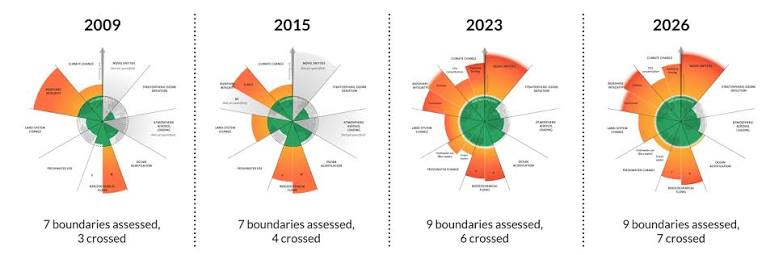
\includegraphics[width=.9\textwidth]{pics/pb_trangression.png}\par
  \vspace{6pt}\raggedright\small
  Each assessment has found more boundaries crossed: from 3 in 2009 to 7 today. AI data centres press on
  several of them: climate through electricity (O1); freshwater, novel entities and biosphere
  integrity through cooling water, e-waste and mining (O2).
  \src{Graphic: Stockholm Resilience Centre, \emph{Planetary boundaries} (stockholmresilience.org). Assessments: Rockström et al.\ (2009); Steffen et al.\ (2015); Richardson et al.\ (2023); Planetary Health Check.}
  \note{%
    \NoteKey{The planet is already outside most of its safe limits, so any new pressure matters.}
    \NoteSlide{The Stockholm Resilience Centre's charts for 2009, 2015, 2023 and 2026. Each wedge is one boundary: the green
    centre is the safe zone, orange to red means crossed. The count rose from 3 crossed (of 7 assessed) to 7 (of 9).}
    \NoteWhy{It sets the frame for the talk: which of these boundaries do AI data centres press on, and at what scale?}
    \NoteSay{30}{The planetary-boundaries framework sets nine limits on how far we can push the Earth system before risking
    abrupt change. Every new assessment has found more of them crossed: three in 2009, seven today. Our question is which
    of these AI data centres press on: climate through their electricity, freshwater through cooling and power plants,
    and novel entities and the biosphere through e-waste and mining. We come back to this as a matrix at the end.}
    \begin{NoteAsk}
      \item \emph{Did data centres cause this?} No. This is a global assessment of all human activity; we only map AI's
        pathways onto it.
    \end{NoteAsk}
  }
\end{frame}

\begin{frame}{Small globally, but highly concentrated}
  \begin{itemize}\footnotesize
    \item The US (45\%), China (25\%) and Europe (15\%) use 85\% of data-centre electricity (415 TWh, 2024);
      tracked AI capacity is even more concentrated: 83\% of 15 GW is in the US
    \item So impacts fall on particular \textbf{grids, basins and communities}. One quarter of data centres sit in
      water-stressed areas, but that count ignores \textbf{size} and \textbf{water use}
  \end{itemize}
  \centering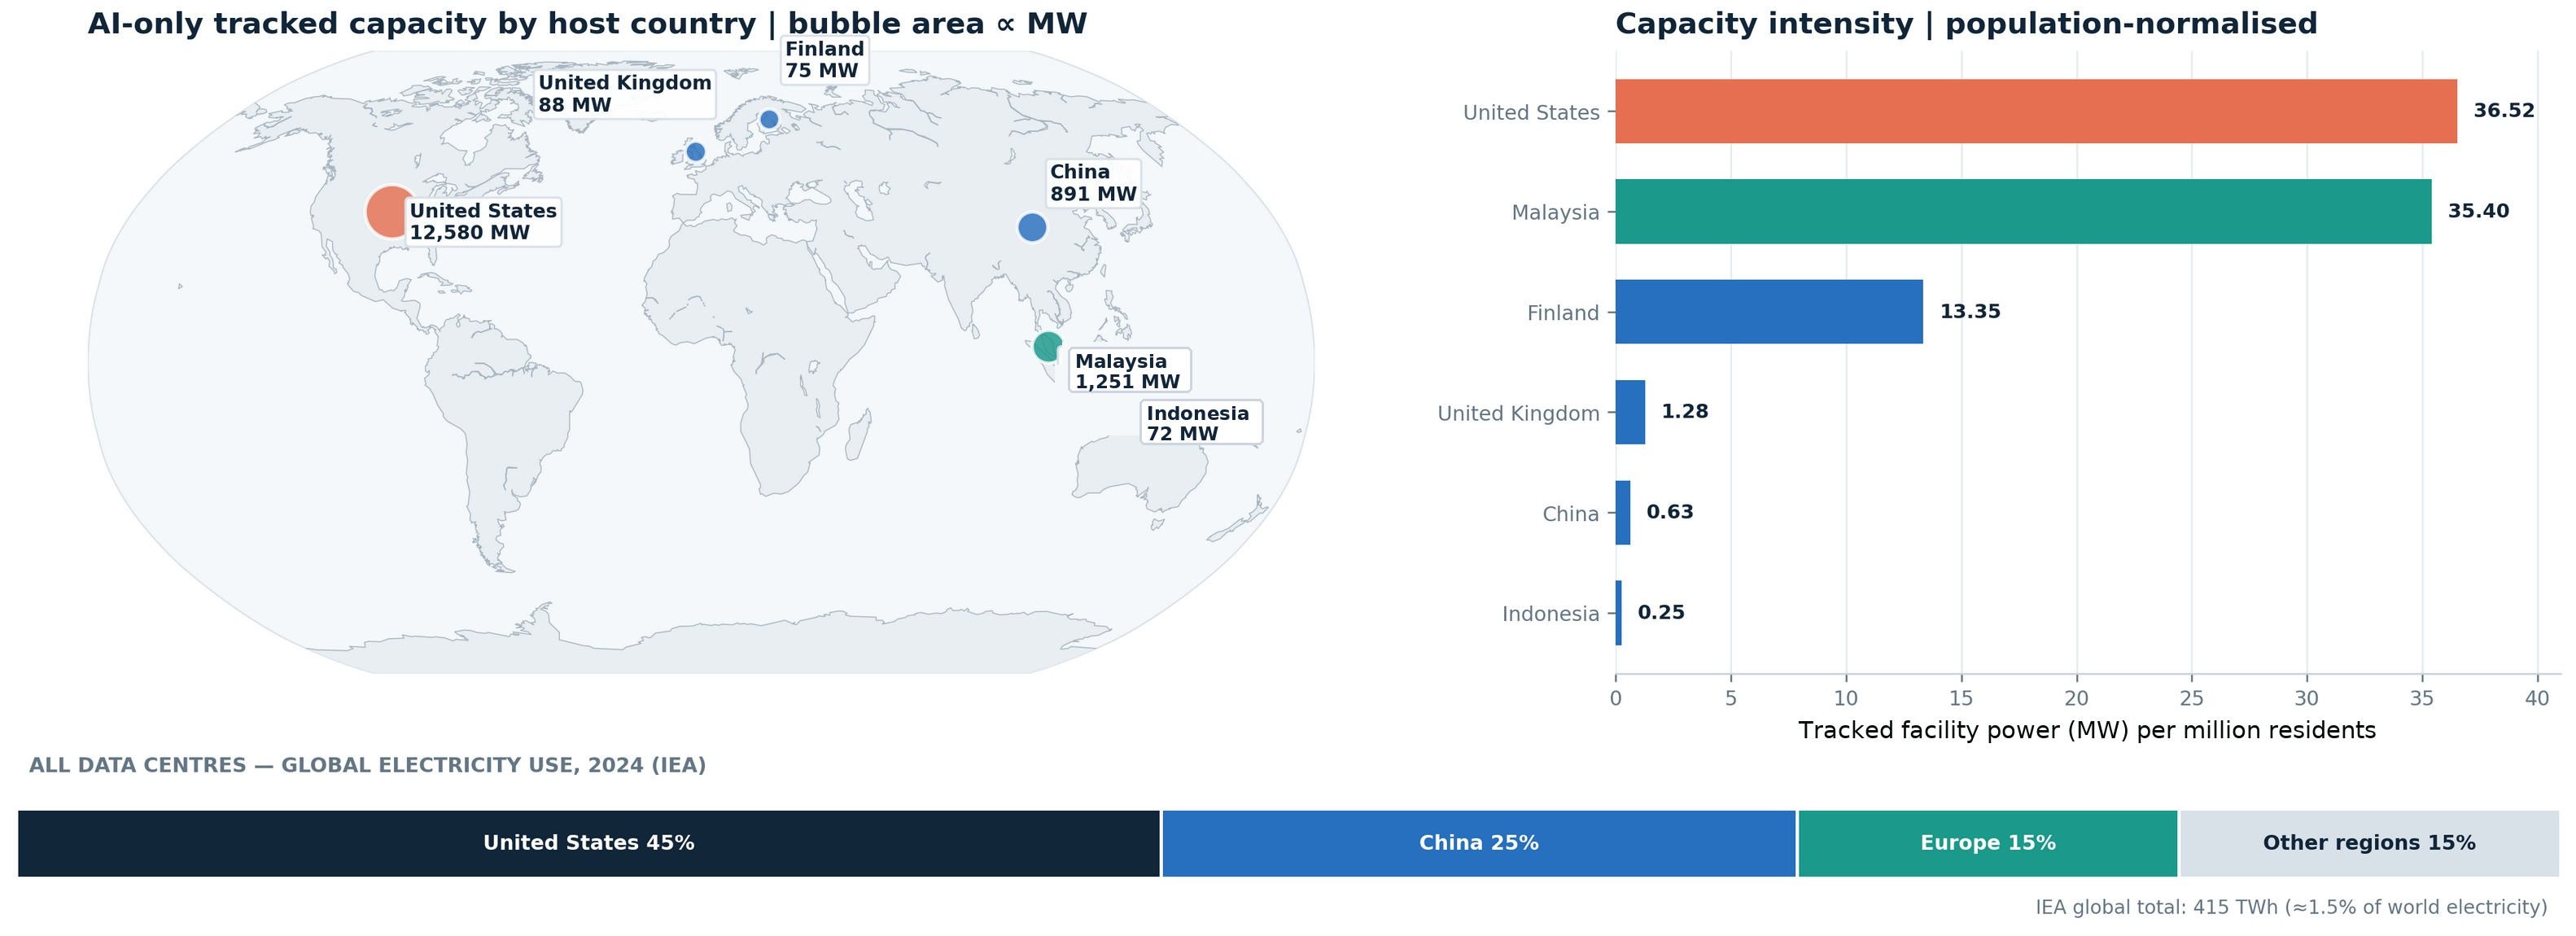
\includegraphics[width=.8\textwidth]{pics/aditya/capacity_map_crop.png}
  \src{IEA (2025) \emph{Energy and AI}; Epoch AI (2026); UN DESA \emph{World Population Prospects 2024}; Rosa et al.\ (2026). Two denominators: IEA covers all data-centre electricity; Epoch covers tracked AI sites only.}
  \note{%
    \NoteKey{Data-centre electricity, and AI capacity even more, sits in very few countries.}
    \NoteSlide{Left map: bubbles show tracked AI data-centre capacity by country (US 12,580 MW, Malaysia 1,251, China 891).
    Right bars: capacity per million residents; the US and Malaysia are far ahead. Bottom bar: the IEA's split of
    \emph{all} data-centre electricity: US 45\%, China 25\%, Europe 15\%.}
    \NoteWhy{Two different datasets, same message. The IEA covers all data centres; Epoch AI covers 96 large AI sites.}
    \NoteSay{45}{Globally data centres are small, but they are concentrated. Three regions, the US, China and Europe, use
    85\% of data-centre electricity. For AI capacity it is even more extreme: 83\% of the 15 gigawatts we track is in the
    US. So the impacts fall on particular grids, basins and communities. A 2026 study found that a quarter of data
    centres sit in water-stressed areas, but it counts sites, not their size or water use. That is the gap we fill.}
    \begin{NoteAsk}
      \item \emph{Why is Malaysia so high per person?} Several large AI sites in Johor, next to Singapore, and a small
        population.
    \end{NoteAsk}
  }
\end{frame}

\begin{frame}{Three phases since 1950, and one puzzle}
  \centering
  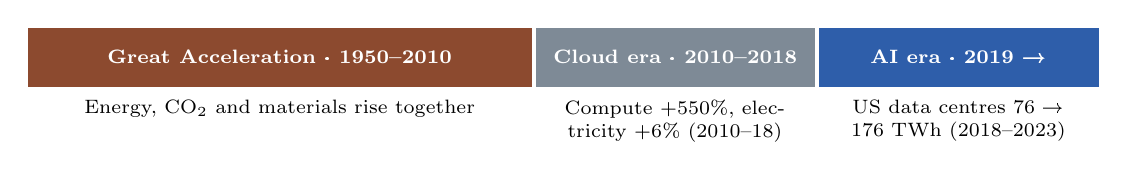
\begin{tikzpicture}[x=1cm,y=1cm]
    \fill[phaseGA]    (0,0)    rectangle (6.4,.75) node[midway,white,font=\scriptsize\bfseries] {Great Acceleration · 1950–2010};
    \fill[phaseCloud] (6.45,0) rectangle (10.0,.75) node[midway,white,font=\scriptsize\bfseries] {Cloud era · 2010–2018};
    \fill[phaseAI]    (10.05,0) rectangle (13.6,.75) node[midway,white,font=\scriptsize\bfseries] {AI era · 2019 →};
    \node[below,font=\scriptsize,text width=6cm,align=center]   at (3.2,-.05)  {Energy, CO\textsubscript{2} and materials rise together};
    \node[below,font=\scriptsize,text width=3.4cm,align=center] at (8.22,-.05) {Compute +550\%, electricity +6\% (2010–18)};
    \node[below,font=\scriptsize,text width=3.4cm,align=center] at (11.82,-.05){US data centres 76 → 176 TWh (2018–2023)};
  \end{tikzpicture}
  \vspace{22pt}

  {\large\bfseries Why did cloud growth leave energy use almost flat,\\
  while AI growth does not?\par}
  \vspace{10pt}
  {\scriptsize\color{muted} In this project, \emph{AI} means data-centre infrastructure.\par}
  \src{Masanet et al.\ (2020) \emph{Science}; Shehabi et al.\ (2024) LBNL; Steffen et al.\ (2015)}
  \note{%
    \NoteKey{Data centres grew for years with little extra energy; AI broke that pattern.}
    \NoteSlide{A timeline of three phases with one fact each. Great Acceleration: energy, CO\textsubscript{2} and materials
    rise together. Cloud era: compute instances +550\% but electricity only +6\% (2010--18). AI era: US data-centre
    electricity 76 $\to$ 176 TWh (2018--2023).}
    \NoteWhy{This is the puzzle the talk answers.}
    \NoteSay{40}{We frame the project in three phases since 1950. In the Great Acceleration, energy, emissions and materials
    all rose together. In the cloud era, the number of computing instances rose by 550\%, yet data-centre electricity
    rose only 6\%. In the AI era, US data-centre electricity more than doubled in five years. So our question is: why
    did cloud growth leave energy almost flat, while AI growth does not?}
    \begin{NoteAsk}
      \item \emph{Why does the AI era start in 2019?} A framing choice from our plan. The data on slide 18 put the jump in
        compute in 2011 and the jump in electricity around 2018, so the boundary is approximate.
    \end{NoteAsk}
  }
\end{frame}

% 2 · Objectives
\section{Objectives}

\begin{frame}{Broad objective: a diagnosis, by scale of impact}
  \vfill
  \begin{center}
    \begin{minipage}{.82\textwidth}
      \large Whether, where, and at what scale AI data centres put pressure on planetary
      boundaries, as a basis for \textbf{responses matched to each scale of impact}.
    \end{minipage}
  \end{center}
  \vfill
  \centering
  \bignum{Whether}{Is the pressure real\\and growing?}\hfill
  \bignum{Where}{Which grids, basins\\and communities?}\hfill
  \bignum{Scale}{Local, regional\\or global?}
  \vfill
  \note{%
    \NoteKey{We diagnose whether, where and at what scale AI data centres press on planetary boundaries.}
    \NoteSlide{The aim, then three questions. \emph{Whether}: is the pressure real and growing? \emph{Where}: which grids,
    basins and communities? \emph{Scale}: local, regional or global?}
    \NoteWhy{The scale decides who has to respond: a town council, a river-basin or grid authority, or a global agreement.}
    \NoteSay{25}{Our broad objective is a diagnosis: whether AI data centres put real pressure on planetary boundaries,
    where that pressure lands, and at what scale, so that responses can be matched to each scale.}
  }
\end{frame}

\begin{frame}{Specific objectives}{}
  {\footnotesize\renewcommand{\arraystretch}{1.35}
  \begin{tabularx}{\textwidth}{@{}>{\bfseries\raggedright\arraybackslash}p{2.7cm}
    >{\raggedright\arraybackslash}p{2.5cm} >{\raggedright\arraybackslash}X@{}}
    \toprule
    & Earth sphere & What we measure \\
    \midrule
    O1\enspace Energy and carbon & Atmosphere
      & Regional capacity, electricity use and grid carbon; growth rates across the three
        phases; why the cloud era stayed flat while the AI era does not \\
    O2\enspace Materials, water and waste & Hydrosphere, lithosphere
      & Water-stress exposure of capacity and nearby people; water use and sources; geography
        of critical minerals and e-waste \\
    O3\enspace Economy, politics and society & Anthroposphere
      & How unevenly capacity is spread relative to population; local opposition;
        supply-chain concentration \\
    O4\enspace Synthesis & All
      & Findings placed on the planetary and safe-and-just boundaries, classified as local,
        regional or global \\
    \bottomrule
  \end{tabularx}}
  \src{Sakschewski et al.\ (2025); Rockström et al.\ (2023) \emph{Nature}}
  \note{%
    \NoteKey{Four objectives, one per part of the Earth system, plus a synthesis.}
    \NoteSlide{O1 energy and carbon (atmosphere). O2 materials, water and waste (hydrosphere = water; lithosphere = rock and
    minerals). O3 economy, politics and society (anthroposphere = the human sphere). O4 synthesis: everything placed on the
    planetary boundaries and sorted into local, regional or global.}
    \NoteWhy{Each later results section answers one of these rows.}
    \NoteSay{30}{We split the work into four objectives. O1 looks at electricity and carbon, and why the cloud era stayed
    flat. O2 looks at water stress, water use, minerals and e-waste. O3 looks at how unevenly capacity is spread and at
    local opposition. O4 puts all of it on the planetary boundaries, by scale.}
    \begin{NoteAsk}
      \item \emph{What are ``safe-and-just'' boundaries?} Rockström et al.\ (2023) add a justice test: limits set so that
        people are not significantly harmed, not only so that Earth stays stable.
    \end{NoteAsk}
  }
\end{frame}

% 3 · Data and methods
\section{Data and methods}

\begin{frame}{Datasets}{}
  {\scriptsize\renewcommand{\arraystretch}{1.0}
  \begin{tabularx}{\textwidth}{@{}>{\bfseries}l >{\raggedright\arraybackslash}X@{}}
    \toprule
    Theme & Sources \\
    \midrule
    Sites and capacity & Epoch AI data centres (MW, timelines; 96 sites), geocoded with OpenStreetMap \\
    Electricity and efficiency & IEA (2025) global and regional; LBNL US 2014–2023; Masanet global 2010–2018; Uptime PUE survey 2007–2025 \\
    Carbon & Ember grid carbon intensity by country (2024) \\
    Water & WRI Aqueduct 4.0 (baseline, 2030, 2050); WUE, PUE and grid water-intensity ranges (de Vries-Gao 2026); city records and news reports (case studies) \\
    Population & GHSL population grid (people near sites); UN World Population Prospects 2024 (capacity per person) \\
    Materials and waste & USGS Mineral Commodity Summaries 2026; Global E-waste Monitor 2024 \\
    Planetary boundaries & Stockholm Resilience Centre; Planetary Health Check 2025; Earth3 thresholds (Collste et al.\ 2018); Great Acceleration framing (Steffen et al.\ 2015) \\
    Society & Data Center Watch Q1 2026 (US); EJAtlas grievance categories; our two case studies \\
    \bottomrule
  \end{tabularx}}
  \par\smallskip
  {\scriptsize\textbf{Changes from the plan:} Epoch AI sites only (no all-data-centre layer or footprint model); 2 case
  studies, not 3–4 clusters; location quotients and country Gini in the report; per-internet-user Gini and a dispute
  catalogue not done; Great Acceleration shown with world energy only.\par}
  \note{%
    \NoteKey{Every number comes from a named public dataset or from our own scripts.}
    \NoteSlide{Sources by theme. The main ones: Epoch AI (96 AI data centres with power in MW, today and planned); IEA, LBNL
    and Masanet (electricity); Uptime Institute (PUE); Ember (grid carbon); WRI Aqueduct (water stress); GHSL (a 1 km
    population grid); USGS (minerals); the Global E-waste Monitor; Data Center Watch (opposition).}
    \NoteWhy{Epoch tracks only large AI sites, not all data centres, so each slide says which group a number refers to.}
    \NoteSay{30}{These are our datasets. The backbone is Epoch AI's database of 96 AI data centres with their power today
    and planned to 2030. Around it we use standard sources: the IEA and Lawrence Berkeley Lab for electricity, WRI's
    Aqueduct for water stress, the EU's population grid, and the US Geological Survey for minerals.}
    \begin{NoteAsk}
      \item \emph{Why only Epoch's sites?} It is the only open dataset with power and build timelines for each AI site.
    \end{NoteAsk}
  }
\end{frame}

\begin{frame}{Methods 1–2: where the capacity sits, and how unevenly}
  \begin{columns}[T,onlytextwidth]
    \column{.48\textwidth}
    \textbf{1\enspace Spatial overlay}
    \begin{itemize}\small
      \item 96 Epoch AI sites with reported MW (today and planned); geocode addresses (OpenStreetMap)
      \item Join to Aqueduct basins; count people within 25 and 50 km (GHSL grid)
      \item Output: \textbf{size-weighted} share of capacity in high water stress, now and in 2030/2050
    \end{itemize}
    \column{.48\textwidth}
    \textbf{2\enspace Inequality}
    \begin{itemize}\small
      \item Location quotient of capacity $C$ against population $P$ (in the report):
    \end{itemize}
    \[ LQ_i = \frac{C_i / C}{P_i / P} \]
    \begin{itemize}\small
      \item Lorenz curve and Gini coefficient of capacity per person (seven country groups)
    \end{itemize}
  \end{columns}
  \note{%
    \NoteKey{Put each site on a map, read its basin's water stress and count the people nearby; then measure how unevenly
    capacity is spread.}
    \NoteSlide{Method 1, spatial overlay: find each site's coordinates, look up its river basin in Aqueduct, count people
    within 25 and 50 km. The key output is the share weighted by MW, not just a count of sites. Method 2, inequality: the
    location quotient (a country's share of capacity $\div$ its share of population; above 1 = more than its share), and
    the Lorenz curve and Gini (0 = perfectly even, 1 = everything in one place).}
    \NoteSay{35}{Method one is a map overlay: each data centre goes onto the water-stress map, and we weight by size, so a
    2-gigawatt campus counts more than a small site. We also count the people living nearby. Method two measures
    inequality, comparing each country's share of capacity with its share of the world's people.}
    \begin{NoteAsk}
      \item \emph{Where are the location quotients?} The country table with them comes in the final report; slide 5 shows
        capacity per person, the same idea.
    \end{NoteAsk}
  }
\end{frame}

\begin{frame}{Methods 3–4: how much water, and how fast it grows}
  \begin{columns}[T,onlytextwidth]
    \column{.48\textwidth}
    \textbf{3\enspace Water-use range}
    \[ W_{\text{direct}} = E_{\text{IT}} \times \text{WUE} \]
    \[ W_{\text{indirect}} = E_{\text{IT}} \times \text{PUE} \times WI_{\text{grid}} \]
    {\small Low and high bounds from published WUE, PUE and generation water-intensity ranges.\par}
    \column{.48\textwidth}
    \textbf{4\enspace Standardised growth}
    \[ \ln y_t = a + bt \]
    \[ r = e^{b}-1, \qquad T_2 = \frac{\ln 2}{b} \]
    {\small 95\% intervals where annual data exist; observed and projected years kept separate.
    A two-segment fit tests where the breakpoints fall in the long series (world energy, AI compute).\par}
  \end{columns}
  \note{%
    \NoteKey{We estimate water from electricity, and measure growth as percent per year and doubling time.}
    \NoteSlide{Method 3: direct water = computer energy $\times$ WUE (litres evaporated on site per kWh); indirect water =
    the building's energy $\times$ the water evaporated per kWh at power plants. Low and high bounds come from published
    ranges. Method 4: fit a straight line to the logarithm of the data. Its slope gives the annual growth $r$ and the
    doubling time $T_2$, with 95\% intervals where yearly data exist; a two-segment fit finds where the trend breaks.}
    \NoteWhy{Rule of thumb: doubling time $\approx$ 70 $\div$ growth in \% (7\% a year $\to$ about 10 years).}
    \NoteSay{35}{Method three estimates water from electricity: on-site cooling water, plus the water evaporated at power
    plants. We give a low and a high value, because published values vary a lot. Method four turns every trend into a
    growth rate and a doubling time, so the three phases can be compared on one scale.}
  }
\end{frame}

\begin{frame}{Method 5: case studies and synthesis}
  \begin{columns}[T,onlytextwidth]
    \column{.44\textwidth}
    \textbf{Two contrasting cases}
    \begin{itemize}\small
      \item Google Mesa, Arizona: on our map, extremely high stress
      \item Google–AdaniConneX Visakhapatnam, India: planned 1 GW, not yet in the Epoch data
    \end{itemize}
    \smallskip
    {\small For each: water source and distance, local reaction, and our own estimate, from news
    reports and official documents.\par}
    \medskip
    {\small All results feed one matrix: \textbf{planetary boundary × scale of impact}.\par}
    \column{.52\textwidth}
    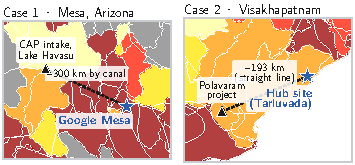
\includegraphics[width=\linewidth]{figs/case_locator.pdf}\par\smallskip
    {\scriptsize\color{muted} Star: data centre. Triangle: its water source. Background: Aqueduct
    baseline water stress (same colours as the results map).\par}
  \end{columns}
  \note{%
    \NoteKey{Two contrasting case studies, and one matrix that pulls everything together.}
    \NoteSlide{Google in Mesa, Arizona (a desert city, on our map, extremely high stress) and Google with AdaniConneX in
    Visakhapatnam, India (planned 1 GW, not yet in Epoch's data). On the map: star = data centre, triangle = its water
    source, colours = water stress. Mesa's river water travels about 300 km by canal; Vizag's promised source, Polavaram,
    is about 190 km away.}
    \NoteWhy{Totals hide places. Case studies show what the numbers mean on the ground.}
    \NoteSay{30}{Method five is two case studies, one in a US desert city and one in an Indian port city, built from news
    reports and official records. For each we look at where the water comes from, how far it travels, how people reacted,
    and our own estimate. Everything then feeds one matrix: planetary boundary by scale of impact.}
  }
\end{frame}

% 4 · Results. One \subsection per objective; each gets a light divider.
% Frame titles are the EXPECTED claims from the plan. Rewrite them as the actual findings.
\section{Results}

% ================================================================ O1
\subsection{O1 · Energy and carbon}

\begin{frame}{US data-centre electricity growth rose from 7\% to 18\% a year}
  \centering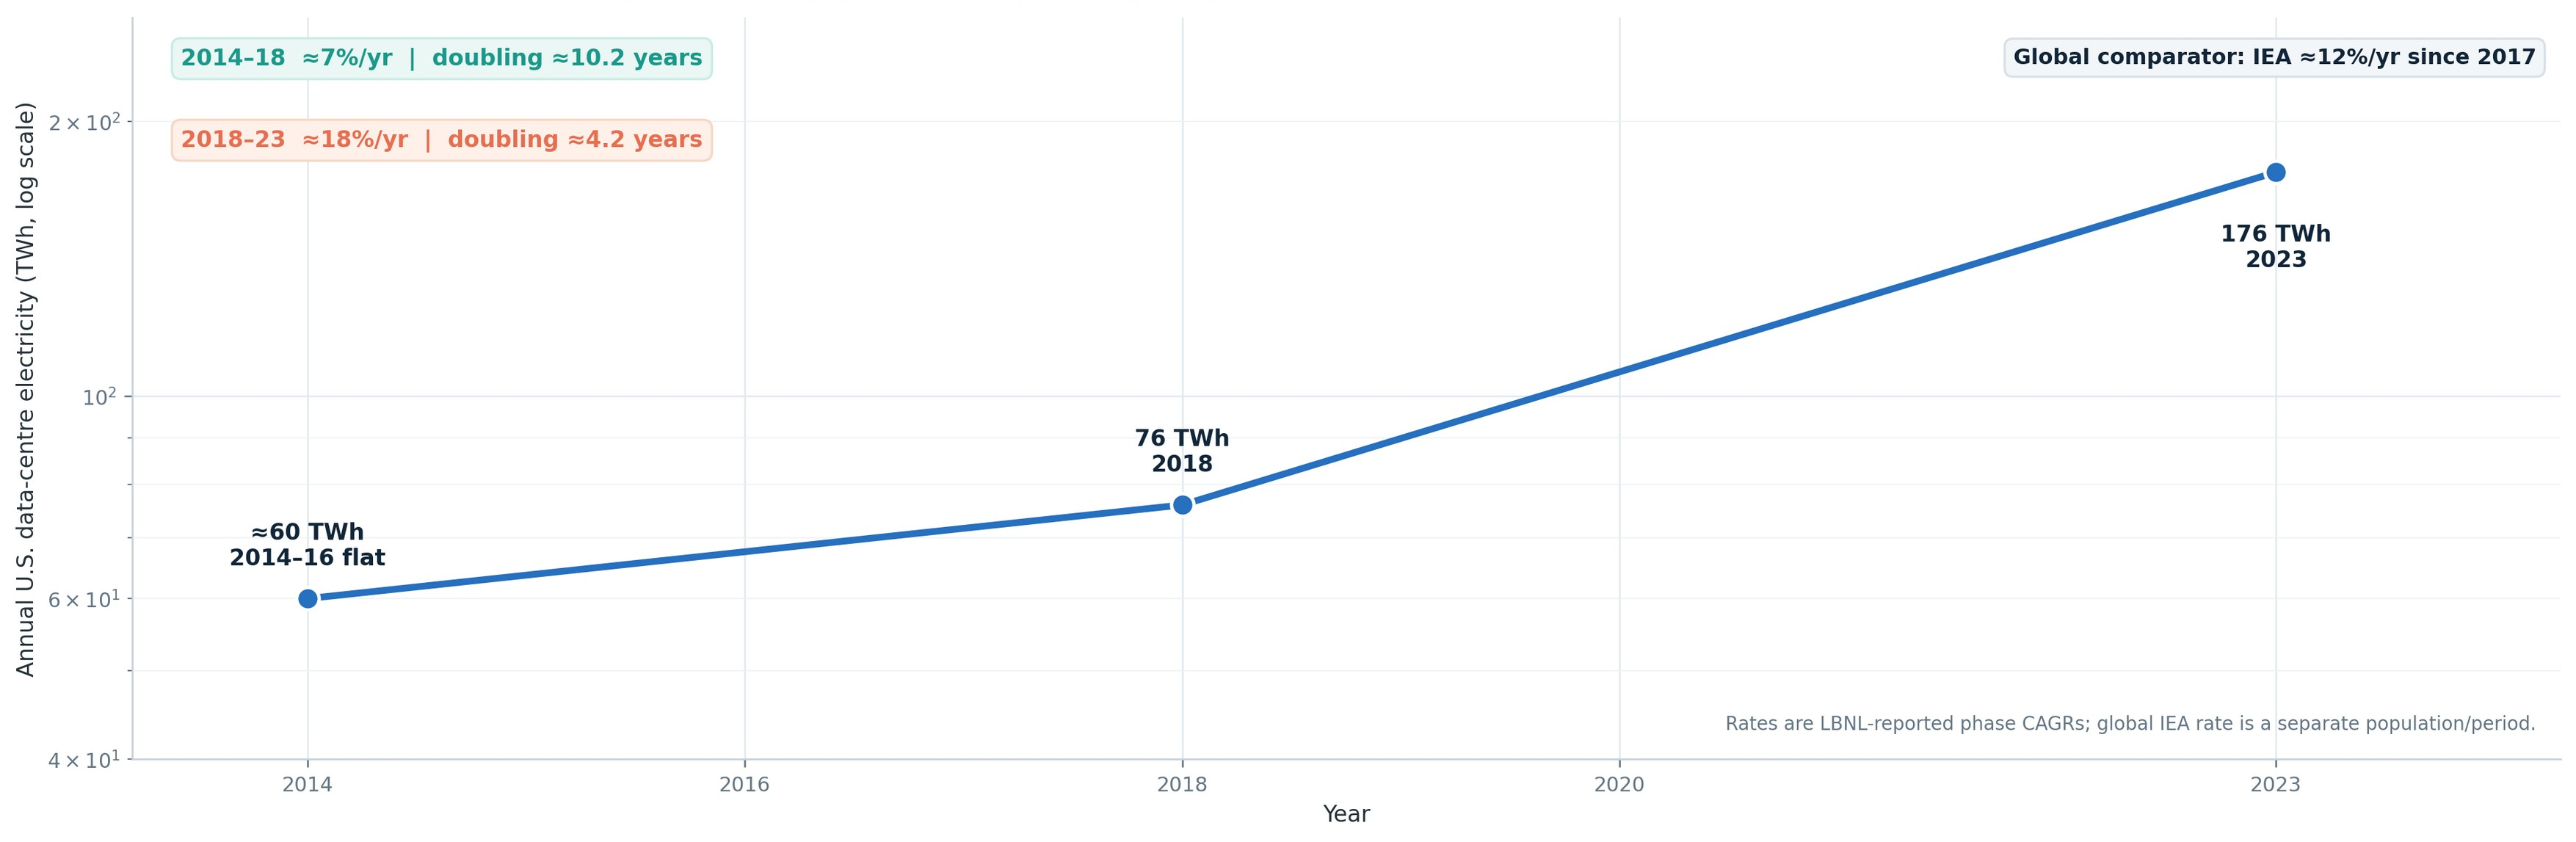
\includegraphics[width=.88\textwidth]{pics/aditya/electricity_growth_crop.png}\par\smallskip
  \raggedright
  \begin{columns}[T,onlytextwidth]
    \column{.56\textwidth}
    {\scriptsize\renewcommand{\arraystretch}{1.25}
    \begin{tabular}{@{}lrr@{}}
      \toprule
      Phase (US, LBNL) & r (\%/yr) & $T_2$ (yr) \\
      \midrule
      \textcolor{phaseCloud}{Cloud, 2014–18 ($\approx$60 → 76 TWh)} & $\approx$7 & $\approx$10.2 \\
      \textcolor{phaseAI}{AI, 2018–23 (76 → 176 TWh)} & $\approx$18 & $\approx$4.2 \\
      \bottomrule
    \end{tabular}\par}
    \column{.4\textwidth}
    {\scriptsize The doubling time fell from about 10 to about 4 years. Globally the IEA estimates
    $\approx$12\%/yr since 2017: a separate series, not spliced in.\par}
  \end{columns}
  \src{Shehabi et al.\ (2024) LBNL-2001637 (growth rates as stated in its executive summary); IEA (2025) \emph{Energy and AI}}
  \note{%
    \NoteKey{US data-centre electricity growth jumped from about 7\% a year to about 18\% a year.}
    \NoteSlide{A line on a log scale, so a steeper line means faster growth: $\approx$60 TWh in 2014--16, 76 TWh in 2018,
    176 TWh in 2023 (Lawrence Berkeley National Lab). The table: cloud era $\approx$7\%/yr, doubling every $\approx$10
    years; AI era $\approx$18\%/yr, doubling every $\approx$4 years.}
    \NoteWhy{The first hard evidence that the AI era breaks the cloud-era plateau.}
    \NoteSay{40}{Here is US data-centre electricity from Lawrence Berkeley National Lab. From 2014 to 2018 it grew about 7\%
    a year, doubling roughly every ten years. From 2018 to 2023 it grew 18\% a year, doubling every four years. That is
    the AI build-out showing up in the electricity data.}
    \begin{NoteAsk}
      \item \emph{And globally?} The IEA estimates about 12\% a year since 2017. That is a different series, so we do not
        splice it in.
    \end{NoteAsk}
  }
\end{frame}

\begin{frame}{One growth table for the three phases}{}
  {\scriptsize\renewcommand{\arraystretch}{1.04}
  \begin{tabularx}{\textwidth}{@{}l X l r r l l@{}}
    \toprule
    Phase & Series & Period & r (\%/yr) & $T_2$ (yr) & 95\% CI & Basis \\
    \midrule
    \textcolor{phaseGA}{\textbf{Great Accel.}} & World primary energy & 1950–2010 & 2.4 & 30 & 28–32 & 48 years \\
    \textcolor{phaseCloud}{\textbf{Cloud era}} & World primary energy & 2010–19 & 1.2 & 58 & 51–66 & 10 years \\
     & Data-centre electricity, world & 2010–18 & 0.7 & $\approx$95 & – & 2 values \\
     & Data-centre electricity, US & 2014–18 & $\approx$7 & $\approx$10 & – & LBNL \\
    \textcolor{phaseAI}{\textbf{AI era}} & Data-centre electricity, US & 2018–23 & $\approx$18 & $\approx$4.2 & – & LBNL \\
     & Data-centre electricity, world & 2024–30 & 14.7 & 5.1 & – & IEA proj. \\
     & AI training compute & 2010–26 & 329 & 0.48 & 0.45–0.51 & 478 models \\
    \bottomrule
  \end{tabularx}}
  \par\smallskip
  {\scriptsize\textbf{Breakpoint test} (two-segment fit): AI compute breaks in \textbf{2011} (doubling 1.7 → 0.5 years).
  World energy: 1974 over 1950–2019, but window-dependent (2011 over 1990–2019); 1950 cannot be tested, as data before
  1965 are decadal. Data-centre electricity: too few points.\par}
  \begin{block}{Our comment}\scriptsize
    Compute took off in 2011, yet data-centre electricity rose only 6\% in 2010–18. PUE stopped improving around 2014;
    the 2018 jump matches AI-server demand (<2 → >40 TWh). Chip efficiency not tested.
  \end{block}
  \src{Our World in Data; Masanet et al.\ (2020); Shehabi et al.\ (2024); IEA (2025); Epoch AI. analysis/growth\_table.py}
  \note{%
    \NoteKey{On one scale, the cloud era is the flat exception, and AI compute is the fastest thing in the table.}
    \NoteSlide{Each row: annual growth $r$, doubling time $T_2$, and a 95\% interval where yearly data exist. World energy
    doubled every 30 years (1950--2010); world data-centre electricity barely moved (2010--18); US data-centre electricity
    doubles every 4 years (2018--23); AI training compute doubles every 6 months.}
    \NoteSay{50}{This puts all three phases on one scale. In the Great Acceleration, world energy doubled about every 30
    years. In the cloud era, data-centre electricity barely moved: plus 6\% in eight years. In the AI era, US
    data-centre electricity doubles every four years. The driver is the bottom row: AI training compute doubles every
    six months. Compute jumped in 2011, yet electricity only turned up around 2018. Building efficiency stopped
    improving around 2014, so the 2018 jump lines up with the arrival of AI servers rather than with PUE.}
    \begin{NoteAsk}
      \item \emph{No intervals for data-centre electricity?} Only a few published points exist; an interval needs a
        yearly series.
      \item \emph{Do the phases start in 1950 and 2010?} Compute breaks in 2011. For world energy it depends on the
        window (1974 over 1950--2019; 2011 over 1990--2019), and 1950 itself cannot be tested.
    \end{NoteAsk}
  }
\end{frame}

\begin{frame}{AI servers' electricity grew more than 20-fold while facility efficiency stalled}
  \centering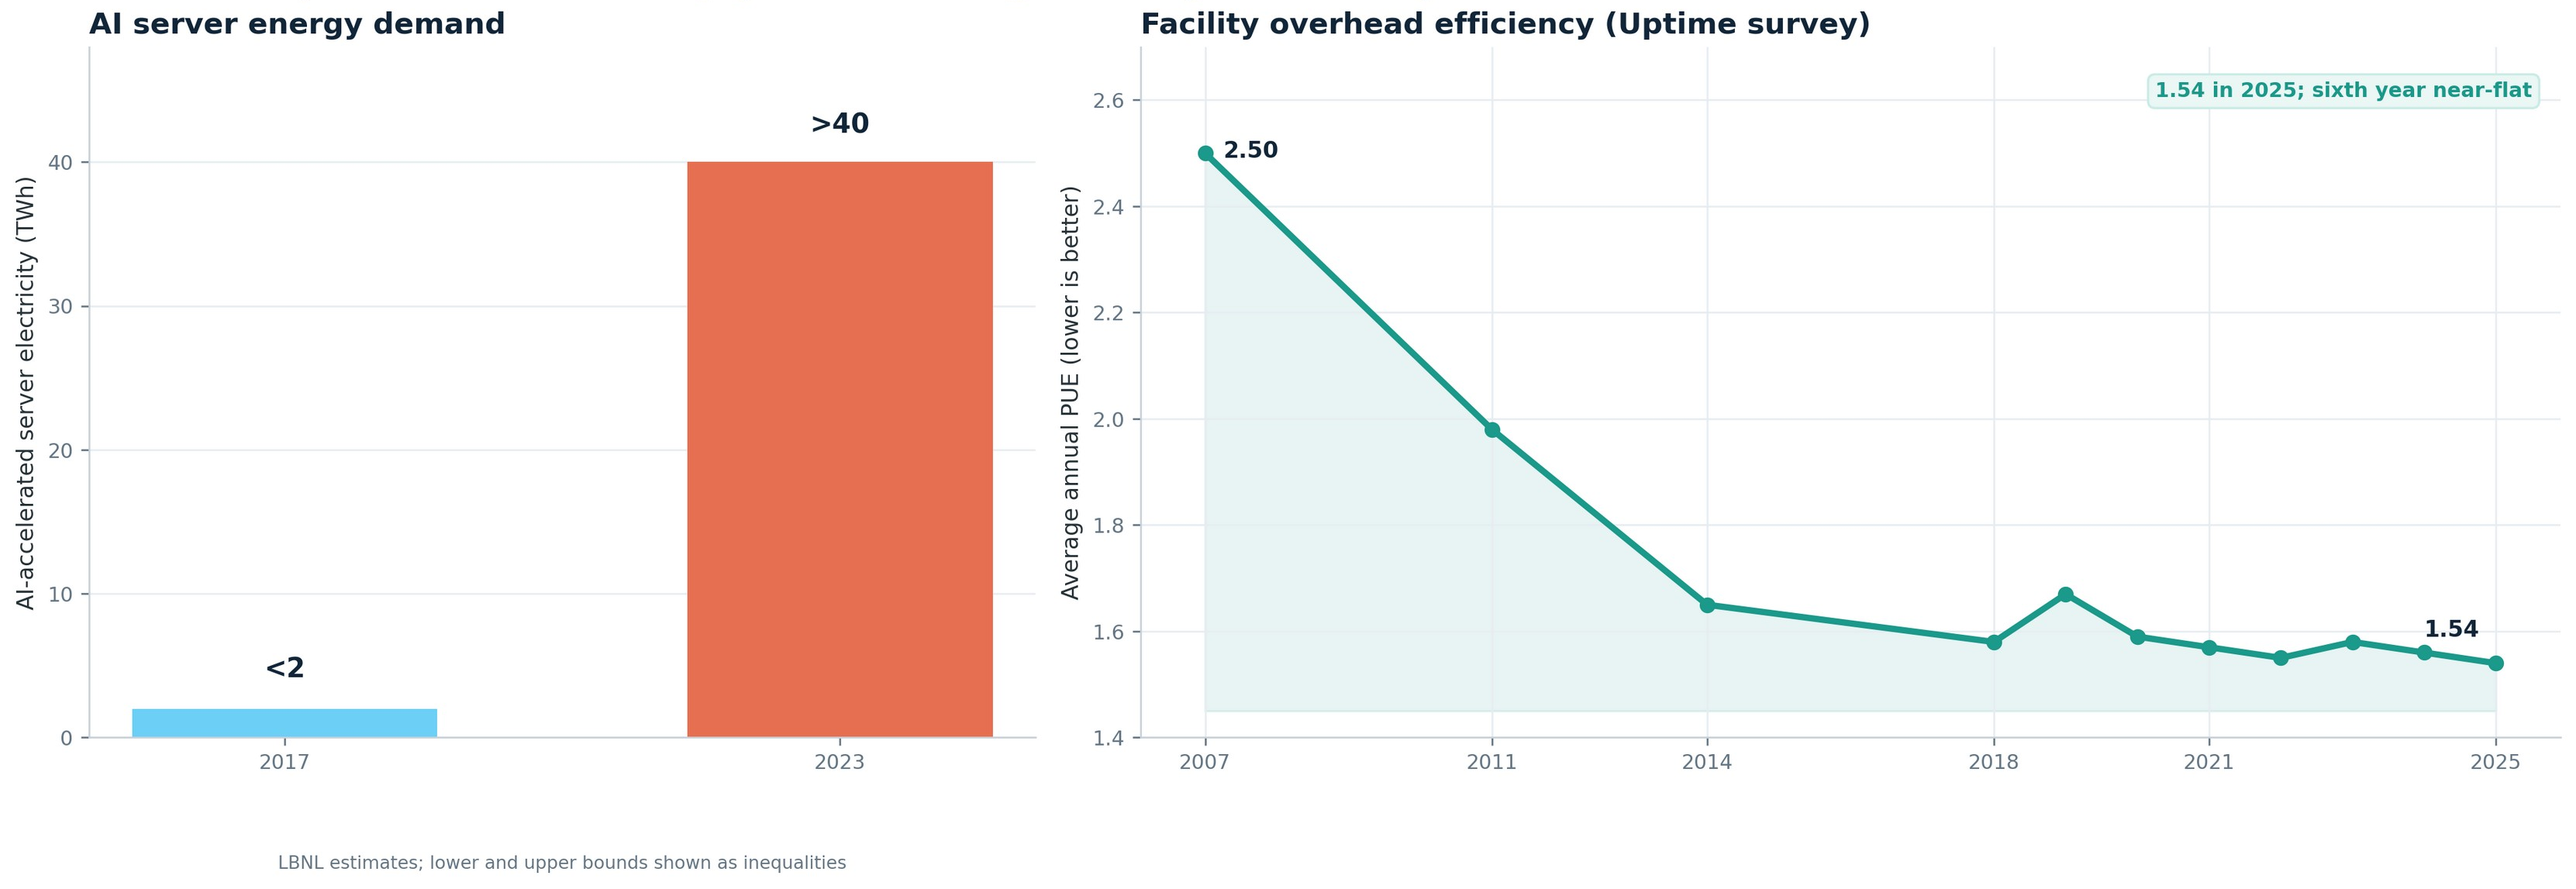
\includegraphics[width=.94\textwidth]{pics/aditya/compute_efficiency_crop.png}\par\smallskip
  \raggedright
  \begin{itemize}\footnotesize
    \item US AI-accelerated servers: under 2 TWh in 2017, over 40 TWh in 2023
    \item Average PUE fell from 2.50 (2007) to 1.65 (2014), then stayed near 1.5 (1.54 in 2025): the easy gains are used up
    \item PUE measures facility overhead, not chip efficiency: we did not test performance per watt
  \end{itemize}
  \src{Shehabi et al.\ (2024) LBNL; Uptime Institute (2025) \emph{Global Data Center Survey}}
  \note{%
    \NoteKey{AI servers' electricity rose more than 20-fold while the easy efficiency gains ran out.}
    \NoteSlide{Left: US AI-accelerated servers used under 2 TWh in 2017 and over 40 TWh in 2023. Right: the average PUE of
    data centres fell from 2.50 (2007) to 1.65 (2014), then stayed around 1.5--1.6 (1.54 in 2025).}
    \NoteWhy{In the cloud era, better buildings (lower PUE) offset growth. That lever is mostly used up, so growth in
    computing now shows up as growth in electricity.}
    \NoteSay{40}{Why did the plateau end? On the left, electricity used by AI servers in the US went from under 2 to over 40
    terawatt-hours in six years. On the right, the efficiency of the buildings: PUE fell fast until 2014 and has been
    almost flat for years. The one-off gains, like better cooling and moving to big efficient sites, are used up.}
    \begin{NoteAsk}
      \item \emph{But chips keep getting more efficient?} Yes. PUE measures the building, not the chip; we did not test
        chip efficiency.
    \end{NoteAsk}
  }
\end{frame}

\begin{frame}{The load sits in three regions; its carbon depends on each grid}
  \centering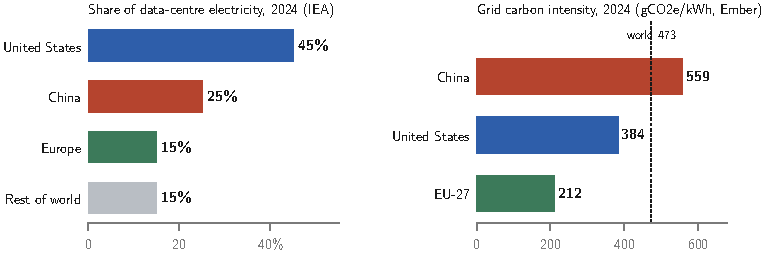
\includegraphics[width=\textwidth]{figs/o1_regional_carbon.pdf}\par\smallskip
  \raggedright
  \begin{itemize}\footnotesize
    \item The same kWh emits about 2.6 times as much CO\textsubscript{2} in China (559 g) as in the EU (212 g)
    \item Electricity is a regional load; carbon is a global impact, set by the local grid mix
    \item The EU-27 is a proxy for the IEA's ``Europe''; intensities are benchmarks, not emission estimates
  \end{itemize}
  \src{IEA (2025) \emph{Energy and AI}; Ember (2026) yearly electricity data, 2024 values (analysis/o1\_regional.py)}
  \note{%
    \NoteKey{Where the electricity is used decides how much CO\textsubscript{2} it emits.}
    \NoteSlide{Left: share of data-centre electricity in 2024: US 45\%, China 25\%, Europe 15\%, rest 15\% (IEA). Right: grid
    carbon intensity in 2024, grams of CO\textsubscript{2} per kWh: China 559, US 384, EU 212; dashed line = world 473
    (Ember).}
    \NoteWhy{The same kWh emits about 2.6 times more CO\textsubscript{2} in China than in the EU. Electricity is a regional
    load; carbon is a global impact.}
    \NoteSay{35}{Electricity use sits in three regions. But what it emits depends on each grid: a kilowatt-hour in China
    emits about two and a half times as much CO\textsubscript{2} as one in the EU. So the electricity is a regional
    problem, for grids and local air, while the carbon adds to a global one.}
    \begin{NoteAsk}
      \item \emph{Are these data-centre emissions?} No: they are grid averages, used as benchmarks. The EU stands in for
        the IEA's ``Europe''.
    \end{NoteAsk}
  }
\end{frame}

% ================================================================ O2
\subsection{O2 · Materials, water and waste}

\begin{frame}{The AI build-out is heading into dry basins}
  \centering
  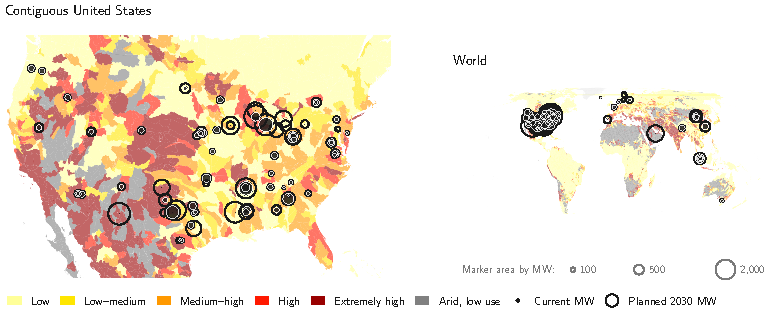
\includegraphics[width=\textwidth]{figs/o2a_sites_water_stress.pdf}\par
  \raggedright\scriptsize 96 AI data centres: 15 GW today, 50 GW planned by 2030. Many of the largest
  planned sites, in West Texas, New Mexico, Abu Dhabi and Inner Mongolia, sit in high or extremely high stress.
  \src{Epoch AI (2026), geocoded via OpenStreetMap; WRI Aqueduct 4.0 baseline water stress}
  \note{%
    \NoteKey{Much of the planned AI build-out is heading into water-stressed river basins.}
    \NoteSlide{Background colour = Aqueduct water stress (yellow = low, dark red = extremely high, grey = arid with little
    use). Filled dot = a site's power today; open ring = planned by 2030. 96 sites: 15 GW today, 50 GW planned.}
    \NoteSay{50}{I worked on water, materials and waste. We took Epoch AI's 96 AI data centres, about 15 gigawatts today and
    50 planned by 2030, and placed each on WRI's water-stress map. Two things stand out. The rings are much bigger than
    the dots: most of this capacity is not built yet. And many of the biggest rings sit in red: Stargate in New Mexico,
    Shackelford and the Texas Panhandle, Stargate UAE in Abu Dhabi, Ulanqab in Inner Mongolia. Not all of them: the
    largest planned site, in Wisconsin, is not stressed. The next slide puts a number on it.}
    \begin{NoteAsk}
      \item \emph{How accurate are the locations?} All 96 were checked against country and state; city-level accuracy is
        enough because basins are tens to hundreds of km across.
      \item \emph{Where is Vizag?} Not in Epoch's data yet; it is case study 2.
    \end{NoteAsk}
  }
\end{frame}

\begin{frame}{By size, 34\% of AI capacity is in stressed basins today, 39–45\% by 2030}
  \begin{columns}[T,onlytextwidth]
    \column{.56\textwidth}
    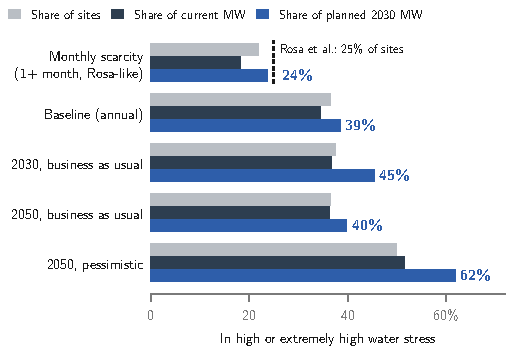
\includegraphics[width=\linewidth]{figs/o2b_count_vs_size.pdf}
    \column{.41\textwidth}
    \begin{itemize}\footnotesize
      \item Today: 37\% of sites, 34\% of MW in high or extremely high stress
      \item Planned MW grows \textbf{3.7×} in stressed basins (3.1× elsewhere): 39\% at today's stress
      \item 45\% at 2030 stress, but most of that step is two Gulf Coast sites near the 40\% line; \textbf{62\%} by 2050, pessimistic
      \item \textbf{21 M} people within 25 km of a stressed site, planned sites included (48 M within 50 km)
      \item Check: our monthly test gives 22\% of sites; Rosa et al.\ 25\%
    \end{itemize}
  \end{columns}
  \src{Epoch AI (2026); WRI Aqueduct 4.0; GHSL GHS-POP 2025; Rosa et al.\ (2026). Annual stress counts all withdrawals, incl.\ power-plant cooling.}
  \note{%
    \NoteKey{Weighted by power, 34\% of AI capacity is in high-stress basins today, 39--45\% by 2030.}
    \NoteSlide{Bars per scenario: grey = share of sites, dark = share of today's MW, blue = share of planned 2030 MW. The
    dashed line is Rosa et al.'s 25\% (a share of sites).}
    \NoteSay{60}{Counting sites treats a 10-megawatt site like a 2-gigawatt campus, so we weight by power. Today, 34\% of AI
    power sits in high-stress basins. Keep today's stress map and look at where new capacity is going: 39\%, because
    capacity in stressed basins grows 3.7 times, against 3.1 elsewhere. With WRI's 2030 projection it is 45\%, but most
    of that step is two big sites in Louisiana and Mississippi sitting just under the 40\% line. In the pessimistic 2050
    case it is 62\%. About 21 million people live within 25 km of a stressed site. As a check, our monthly test gives
    22\% of sites, close to Rosa's 25\%.}
    \begin{NoteAsk}
      \item \emph{Why is 2050 lower than 2030?} The same two Gulf Coast basins fall back below 40\%: a threshold effect.
      \item \emph{Why is Indiana ``high''?} Aqueduct counts all withdrawals, including power-plant cooling water.
    \end{NoteAsk}
  }
\end{frame}

\begin{frame}{Most of the water is used at power plants, not on site}
  \begin{columns}[T,onlytextwidth]
    \column{.56\textwidth}
    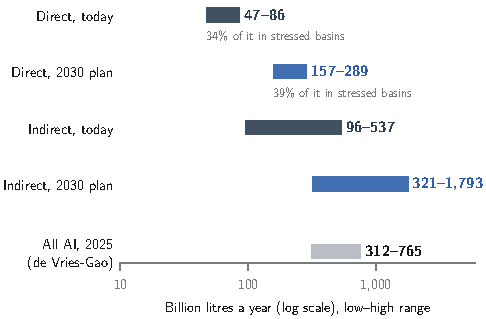
\includegraphics[width=\linewidth]{figs/o2c_water_use.pdf}
    \column{.41\textwidth}
    \begin{itemize}\footnotesize
      \item Today's 15 GW: \textbf{143–624 bn L} a year; the 2030 plan: 478–2,082 bn L
      \item \textbf{67–86\%} of it is indirect, consumed by the power plants
      \item On-site cooling water in stressed basins: 16–30 bn L today, 61–111 bn L by 2030
      \item Reported sites range from 0.001 to 7 L/kWh: cooling design matters more than size
    \end{itemize}
  \end{columns}
  \src{Parameters from de Vries-Gao (2026) \emph{Patterns}: WUE 0.56–1.04 L/kWh, PUE 1.10–1.43, grid 1.04–4.52 L/kWh. Load factor 70–90\% (our assumption). Epoch AI (2026).}
  \note{%
    \NoteKey{Most of the water AI uses is evaporated at power plants, not at the data centre.}
    \NoteSlide{Each bar is a low--high range in billions of litres a year, on a log scale (each gridline is 10$\times$).
    Direct = on-site cooling; indirect = power plants; today and the 2030 plan. Grey = de Vries-Gao's estimate for all
    AI worldwide in 2025. For scale: 1 billion litres $\approx$ 400 Olympic pools.}
    \NoteSay{50}{How much water is that? Today's 15 gigawatts use 143 to 624 billion litres a year; the 2030 plan, 478
    billion to about 2 trillion. The main point: two-thirds to 86\% of that is not at the data centre at all. It
    evaporates at the power plants that feed it. And sites that report water vary by a factor of thousands, from almost
    zero to 7 litres per kWh, so cooling design matters more than size. Our one assumption: sites run at 70 to 90\% of
    their power.}
    \begin{NoteAsk}
      \item \emph{Why such a wide range?} The power-plant factor: 1.04 vs 4.52 litres per kWh in the published sources.
      \item \emph{Consumed or withdrawn?} Consumed (evaporated), on both sides.
    \end{NoteAsk}
  }
\end{frame}

\begin{frame}{Two case studies: a desert city in the US, a port city in India}
  \centering
  \begin{minipage}[t]{.6\textwidth}\centering
    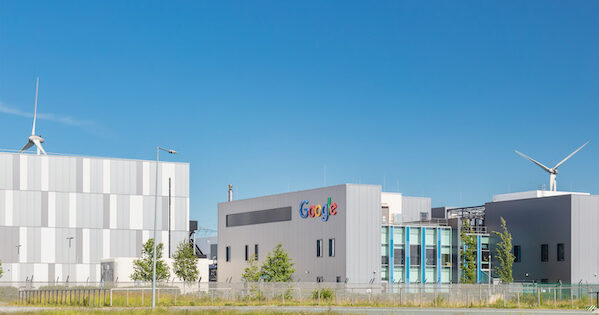
\includegraphics[height=4.3cm]{pics/google_mesa_az.png}\par\smallskip
    {\footnotesize\textbf{Case 1 · Google, Mesa, Arizona}\par}
    {\scriptsize On our map · extremely high water stress\par}
  \end{minipage}\hfill
  \begin{minipage}[t]{.36\textwidth}\centering
    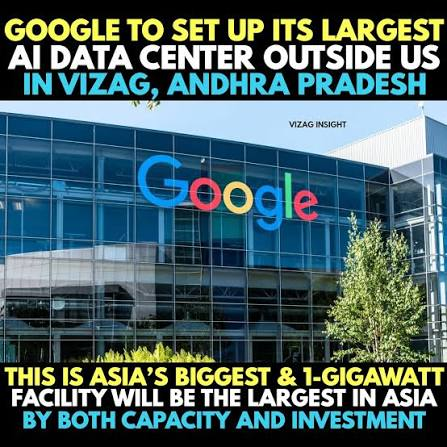
\includegraphics[height=4.3cm]{pics/vishakhapatnam_image.png}\par\smallskip
    {\footnotesize\textbf{Case 2 · Google–AdaniConneX, Visakhapatnam}\par}
    {\scriptsize Planned 1 GW · not yet in the Epoch data\par}
  \end{minipage}
  \src{Left: illustrative photo of a Google data centre, not the Mesa site. Right: announcement as reported on social media (Vizag Insight); the photo is a Google office, not the Vizag site.}
  \note{%
    \NoteKey{Two case studies, chosen to contrast: a US desert city on our map, an Indian port city not yet in the data.}
    \NoteSlide{Two pictures. The left one is a Google data centre, but not the Mesa site. The right one is the announcement
    as it circulated on social media.}
    \NoteSay{20}{Totals hide what happens in one place, so we picked two case studies from official records and news reports:
    a desert city in the US that is on our map, and a port city in India that is not in the data yet.}
  }
\end{frame}

\begin{frame}{Case 1 · Google Mesa: a desert site whose water travels \textasciitilde300 km}
  \begin{columns}[T,onlytextwidth]
    \column{.53\textwidth}
    \begin{itemize}\footnotesize
      \item On our map: 183 MW today, 237 MW planned. Its basin is in \textbf{extremely high} stress;
        withdrawals exceed supply in \textbf{all 12 months}
      \item Google's deal with the city (reported 2020): 1 million gallons a day guaranteed, up to 4 million:
        \textbf{15 million L a day}, 5.5 bn L a year
      \item 2021, Mesa's next data centre (Facebook-linked): Vice Mayor Jenn Duff, the only vote against,
        called data centres ``an irresponsible use of our water''
      \item The canal's river is shrinking: in August 2026 the federal government cut Lower Basin
        allocations by 1.25 million acre-feet a year for 2027–28
    \end{itemize}
    \column{.43\textwidth}
    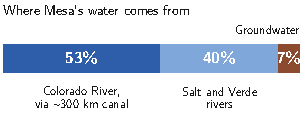
\includegraphics[width=\linewidth]{figs/case_mesa.pdf}\par\smallskip
    \begin{block}{Our comment}\footnotesize
      The stress is local, the source distant: over half of Mesa's water comes by canal from a
      river already being cut.
    \end{block}
  \end{columns}
  \src{City of Mesa water supply page (2026); US Bureau of Reclamation (CAP; news release 21 Aug 2026); Bloomberg (1 Apr 2020); NBC News (19 Jun 2021); Epoch AI; WRI Aqueduct 4.0}
  \note{%
    \NoteKey{A data centre in a desert basin that already uses more water than it gets, fed by a shrinking river 300 km away.}
    \NoteSlide{Facts on the left. The bar shows where Mesa's water comes from: 53\% Colorado River (via the Central Arizona
    Project canal), 40\% Salt and Verde rivers, 7\% groundwater. One acre-foot $\approx$ 1.23 million litres.}
    \NoteSay{60}{Mesa is a suburb of Phoenix. Google's site there is 183 megawatts today, 237 planned. Its basin uses more
    water than it renews in every month of the year. Google's deal with the city, reported in 2020, guarantees a million
    gallons a day and allows up to four million, about 15 million litres. In 2021, when the city approved its next data
    centre, the vice mayor cast the only vote against, calling data centres an irresponsible use of water. More than half
    of Mesa's water is Colorado River water carried about 300 km by canal, and in August 2026 the federal government cut
    Lower Basin allocations by 1.25 million acre-feet a year. The stress is local; the source is distant and shrinking.}
    \begin{NoteAsk}
      \item \emph{Does Google use 4 million gallons a day?} That is the ceiling in the deal; actual use is not disclosed.
    \end{NoteAsk}
  }
\end{frame}

\begin{frame}{Case 2 · Visakhapatnam: a gigawatt AI hub in a city already 15\% short}
  \begin{columns}[T,onlytextwidth]
    \column{.53\textwidth}
    \begin{itemize}\footnotesize
      \item Google with AdaniConneX and Airtel: \textbf{1 GW}, about US\$15 bn; foundation stone laid April 2026 (Tarluvada)
      \item The city receives \textbf{410 of the 480 million L} a day it needs
      \item The environmental clearance does not disclose water use in operation; the state says
        water will come from Polavaram by dedicated pipeline
      \item Google and AdaniConneX say they will air-cool. Residents protest: ``We cannot drink data''
    \end{itemize}
    \column{.43\textwidth}
    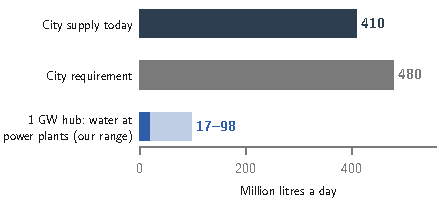
\includegraphics[width=\linewidth]{figs/case_vizag.pdf}\par\smallskip
    \begin{block}{Our comment}\footnotesize
      Our check: medium–high stress basin (20–40\%). Air cooling saves on-site water, but the power
      plants, wherever they are, would still use \textbf{17–98 million L a day}: equal to 4–24\% of the city's supply.
    \end{block}
  \end{columns}
  \src{The Federal (27 Oct 2026); Mongabay India (12 May 2026); Google (Oct 2025). Our estimate uses the slide-24 ranges (US-derived grid water intensity).}
  \note{%
    \NoteKey{A planned 1 GW AI hub in a city that already lacks 15\% of the water it needs.}
    \NoteSlide{Facts on the left. The bar: the city gets 410 million litres a day but needs 480; our estimate for the hub's
    power-plant water is 17--98 million litres a day.}
    \NoteSay{60}{In October 2025 Google announced a 1-gigawatt AI hub in Visakhapatnam with AdaniConneX and Airtel, about 15
    billion dollars. The city already gets only 410 of the 480 million litres a day it needs. The environmental clearance
    does not say how much water the site will use once running; the state says water will come by pipeline from
    Polavaram, about 190 km away; the companies say they will use air cooling. Residents protested: ``We cannot drink
    data.'' Our check: air cooling removes only the on-site water. The power plants, wherever they are, would still evaporate 17 to 98
    million litres a day, equal to 4 to 24\% of what the whole city gets.}
    \begin{NoteAsk}
      \item \emph{Does that come from the city's pipes?} Not necessarily: it compares scale, not the same supply.
      \item \emph{Reports of a 2.51 GW clearance?} Recent press reports it; we use Google's announced 1 GW.
    \end{NoteAsk}
  }
\end{frame}

\begin{frame}{Minerals come from a few countries; e-waste collection is very uneven}
  \centering
  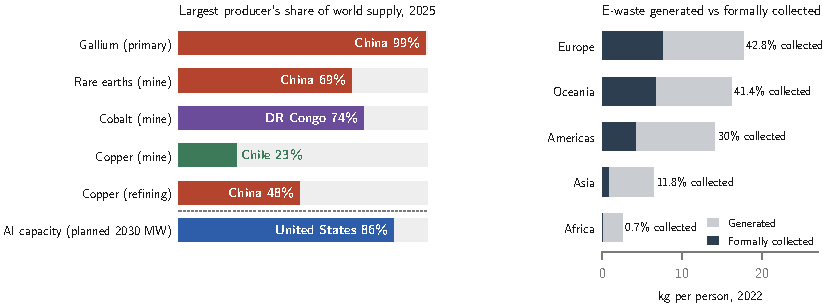
\includegraphics[width=\textwidth]{figs/o2d_materials_ewaste.pdf}\par
  \vspace{4pt}\raggedright\scriptsize Gallium and rare earths come mostly from China and cobalt from DR Congo;
  86\% of planned AI capacity is in the US. China's December 2024 ban on gallium and germanium exports to the
  US is suspended only until 27~Nov~2026. E-waste: 62 Mt in 2022, 22\% formally collected; in Africa, under 1\%.
  \src{USGS Mineral Commodity Summaries 2026; Baldé et al.\ (2024) \emph{Global E-waste Monitor}; Epoch AI (2026)}
  \note{%
    \NoteKey{The minerals come from a few countries, the demand from the US, and e-waste is handled very differently by region.}
    \NoteSlide{Left: the largest producer's share of world supply in 2025 (USGS): China 99\% of gallium (chips, power
    electronics), 69\% of rare earths (magnets), 48\% of refined copper (wiring); DR Congo 74\% of cobalt (batteries).
    Bottom bar: 86\% of planned AI capacity is in the US. Right: e-waste per person in 2022, with the formally collected
    part in dark: Europe 43\%, Africa 0.7\%.}
    \NoteSay{50}{Last, materials and waste. A handful of countries supply the key minerals: China produces almost all
    gallium and most rare earths, DR Congo most cobalt, while the demand sits in the US. And supply can be cut: China's
    ban on gallium and germanium exports to the US is only suspended until 27 November 2026. E-waste ends up in a third
    region: Europe formally collects 43\% of its e-waste, Africa under 1\%. For minerals the impact is displaced, far
    from where the chips are used; for e-waste we can only show that collection is very uneven.}
    \begin{NoteAsk}
      \item \emph{How much of these minerals goes to AI?} The USGS does not break that out; the slide is about
        concentration.
      \item \emph{Does AI e-waste end up in Africa?} We did not trace that: the data cover all electronics.
      \item \emph{Check before presenting:} has the 27 Nov 2026 suspension been extended?
    \end{NoteAsk}
  }
\end{frame}

\begin{frame}{Against a global boundary AI's water barely registers; in a basin it does}
  \small The Earth3 model (Collste et al.\ 2018) tracks freshwater as one global number: withdrawals below
  3,000 km\textsuperscript{3} a year are safe, above 4,000 high-risk.
  \vspace{5pt}

  \centering
  \bignum[phaseAI]{<0.1\%}{of Earth3's safe limit: the 2030 plan uses 0.5–2.1 km\textsuperscript{3} a year}\hfill
  \bignum[phaseAI]{12 of 12}{months a year with withdrawals above supply in Google Mesa's basin}\hfill
  \bignum[phaseAI]{15\% short}{Visakhapatnam gets 410 of the 480 million L a day it needs}
  \vspace{5pt}

  \raggedright
  \begin{block}{Our comment}\footnotesize
    A single global number averages away exactly where the pressure is. AI's water use has to be judged
    basin by basin, and city by city.
  \end{block}
  \src{Collste et al.\ (2018) Earth3 technical notes, p.\,27 (thresholds as in Steffen et al.\ 2015); our estimates, slides 24, 26, 27. Earth3 counts withdrawals; ours is consumption, so withdrawals would be larger.}
  \note{%
    \NoteKey{Against the planet's freshwater limit AI barely registers; in particular basins it does.}
    \NoteSlide{The Earth3 model sets a global freshwater limit: withdrawals under 3,000 km\textsuperscript{3} a year are safe,
    over 4,000 high-risk (1 km\textsuperscript{3} = a trillion litres). Three numbers: $<$0.1\% (the 2030 plan's 0.5--2.1
    km\textsuperscript{3}), 12 of 12 months over supply in Mesa's basin, and Vizag already 15\% short of the water it needs.}
    \NoteWhy{Water cannot move between basins the way CO\textsubscript{2} mixes in the air, so a global total is the wrong
    yardstick for water.}
    \NoteSay{45}{To close my part, back to planetary boundaries. On Earth3's global freshwater scale, the entire 2030 AI plan
    is less than a tenth of a percent: it barely registers. But Mesa's basin already uses more than it gets every month,
    and Visakhapatnam already gets 15\% less water than it needs, before a gigawatt hub arrives. So AI's water has to be
    judged basin by basin. Next: who bears these costs.}
    \begin{NoteAsk}
      \item \emph{So it is not bad globally?} For water, yes, it is small. For carbon, the global total is what counts, and
        it is growing fast (O1).
      \item \emph{Withdrawal vs consumption?} Earth3 counts withdrawals; ours is consumption, so the true share is larger.
    \end{NoteAsk}
  }
\end{frame}

% ================================================================ O3
\subsection{O3 · Economy, politics and society}

\begin{frame}{Tracked AI capacity is far more concentrated than population}
  \centering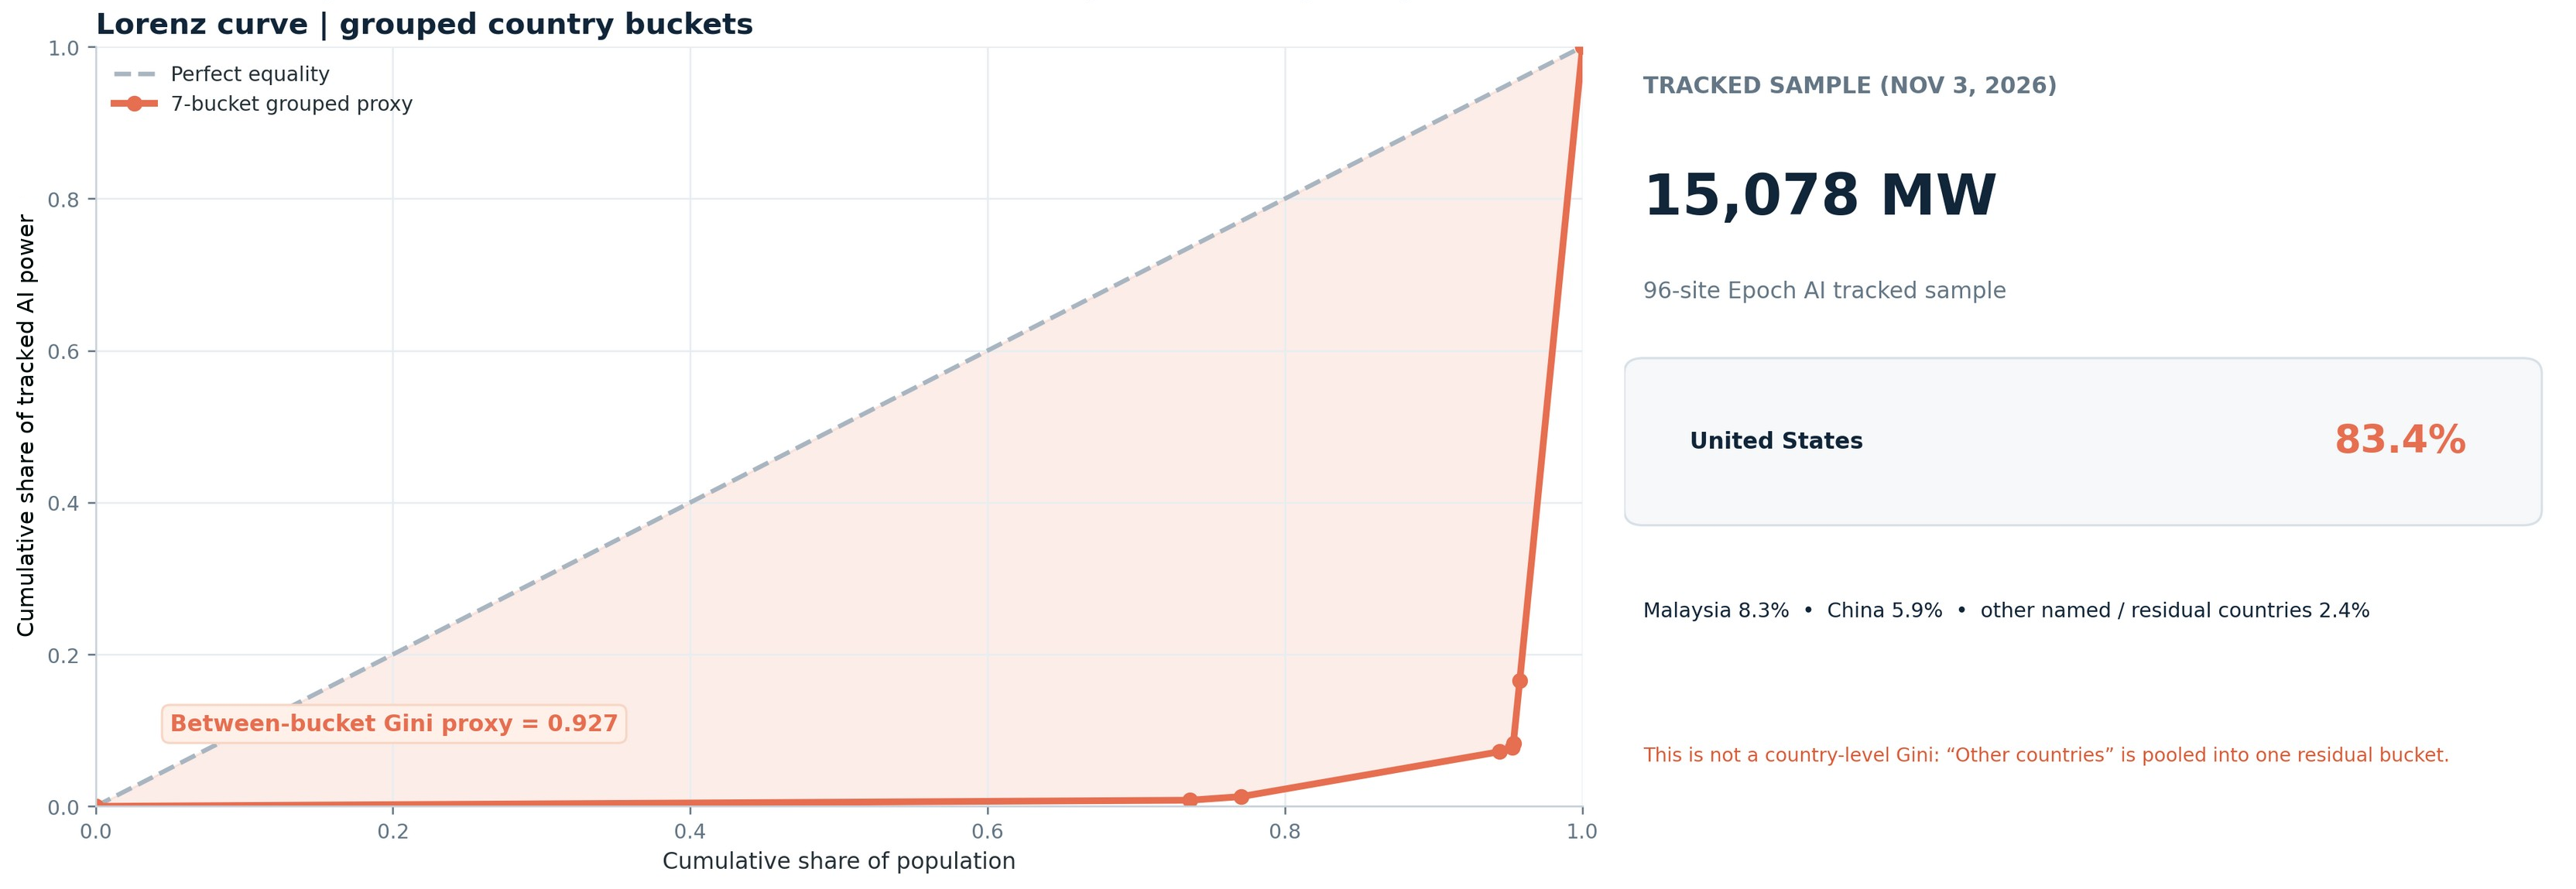
\includegraphics[width=.92\textwidth]{pics/aditya/lorenz_crop.png}\par\smallskip
  \raggedright
  \begin{itemize}\footnotesize
    \item United States 83.4\% of the 15,078 MW tracked; Malaysia 8.3\%; China 5.9\%
    \item Across seven country groups the Gini is \textbf{0.927} (1 = all capacity in one place)
    \item A between-group proxy: pooling ``other countries'' hides inequality within that group
  \end{itemize}
  \src{Epoch AI (2026); UN DESA \emph{World Population Prospects 2024}. Grouping and Gini: project calculation (Aditya).}
  \note{%
    \NoteKey{AI capacity is far more concentrated than people are.}
    \NoteSlide{A Lorenz curve. Horizontal axis: share of the world's population, countries sorted from least to most capacity
    per person. Vertical axis: share of AI capacity. The diagonal is perfect equality; the further the curve sags below
    it, the more unequal. Gini 0.927 (0 = equal, 1 = all in one place). The US holds 83.4\% of 15,078 MW.}
    \NoteWhy{Most of the world hosts almost none of this capacity, so the local costs fall on a few places.}
    \NoteSay{40}{This curve compares where AI capacity is with where people live. If capacity followed population, the curve
    would sit on the diagonal. Instead it hugs the bottom and shoots up at the end: the US alone holds 83\% of what we
    track. Across seven country groups the Gini coefficient is 0.93, close to the maximum.}
    \begin{NoteAsk}
      \item \emph{Why seven groups, not all countries?} A first estimate; pooling ``other countries'' hides inequality inside
        that group. The country-level Gini comes in the report.
    \end{NoteAsk}
  }
\end{frame}

\begin{frame}{Local opposition is rising: \$130 bn of US projects blocked or delayed}
  \centering
  \bignum[phaseAI]{2×}{active opposition groups since\\end-2025, now in 49 US states}\hfill
  \bignum[phaseAI]{75+}{US data-centre projects\\blocked or delayed (Q1 2026)}\hfill
  \bignum[phaseAI]{\$130 bn}{value of the affected\\projects}\par
  \vspace{8pt}
  \raggedright
  {\scriptsize\renewcommand{\arraystretch}{1.15}
  \begin{tabularx}{\textwidth}{@{}>{\bfseries}l X@{}}
    \toprule
    Grievance & What is disputed (tags for coding each case) \\
    \midrule
    Water & Cooling withdrawals, basin stress, competition with households and farms \\
    Power & Grid connection, new generation, electricity bills, fossil lock-in \\
    Noise & Cooling fans, chillers, backup generators \\
    Land & Campus footprint, rezoning, habitat loss, traffic \\
    Jobs & Construction vs permanent jobs; local hiring \\
    \bottomrule
  \end{tabularx}}
  \src{Data Center Watch (2026) \emph{Q1 2026 report}; tags adapted from EJAtlas (Temper et al.\ 2015): a coding framework, not measured totals. Both our cases are about water.}
  \note{%
    \NoteKey{Local resistance is now large enough to block or delay billions of dollars of projects.}
    \NoteSlide{Data Center Watch, US, first quarter of 2026: opposition groups doubled since the end of 2025 and are now in
    49 states; at least 75 projects were blocked or delayed, worth about \$130 billion. The table lists five grievance
    types (water, power, noise, land, jobs) used to code each dispute.}
    \NoteWhy{This is the local scale pushing back. Both our case studies are water disputes.}
    \NoteSay{40}{The local scale is pushing back. In the US, opposition groups doubled in a few months and now exist in 49
    states, and in just the first quarter of 2026 at least 75 projects worth about 130 billion dollars were blocked or
    delayed. The complaints fall into five types: water, power and electricity bills, noise, land, and the jobs promised.}
    \begin{NoteAsk}
      \item \emph{Is there global data?} These figures are US only. The five types follow the EJAtlas categories; a global
        count was not done.
    \end{NoteAsk}
  }
\end{frame}

% ================================================================ O4
\subsection{O4 · Synthesis}

\begin{frame}{Each pressure has its own scale}{}
  {\tiny\renewcommand{\arraystretch}{1.08}
  \begin{tabularx}{\textwidth}{@{}>{\bfseries\raggedright\arraybackslash}p{2.2cm} >{\raggedright\arraybackslash}p{1.45cm} >{\raggedright\arraybackslash}X >{\raggedright\arraybackslash}X >{\raggedright\arraybackslash}X@{}}
    \toprule
    Boundary & Status (2025) & Local & Regional & Global \\
    \midrule
    Climate change & Transgressed & D\enspace Backup generators; construction & \textbf{Q}\enspace Grid intensity 212–559 gCO\textsubscript{2}/kWh & D\enspace Operational and embodied GHG \\
    Freshwater change & Transgressed & \textbf{Q}\enspace 34\% of capacity in stressed basins; Mesa up to 15 M L/day & \textbf{Q}\enspace 67–86\% of water used at power plants & \textbf{Q}\enspace <0.1\% of Earth3's limit: the total hides the hotspots \\
    Land-system change & Transgressed & D\enspace Campus and substation footprint & D\enspace Transmission corridors; mining land & D\enspace Land conversion in the supply chain \\
    Biosphere integrity & Transgressed & D\enspace Habitat effects of sites & D\enspace Mining, river and wetland pressure & D\enspace Cumulative ecosystem pressure \\
    Biogeochemical flows & Transgressed & N & D\enspace Generation, mining and runoff & N \\
    Novel entities & Transgressed & D\enspace Refrigerants, chemicals, exhaust & \textbf{Q}\enspace E-waste collected: 43\% in Europe, 0.7\% in Africa & D\enspace Hazardous material flows \\
    Ocean acidification & Transgressed & N & N & D\enspace Through CO\textsubscript{2} only \\
    Aerosol loading & Safe & D\enspace Diesel and construction particulates & D\enspace Combustion pollution & N \\
    Ozone depletion & Safe & N & N & N \\
    \bottomrule
  \end{tabularx}}
  \par\smallskip
  {\tiny \textbf{Q} quantified in this project\quad D documented pathway, not quantified\quad N not assessed.\quad
  Status is a global assessment, not a finding that data centres caused it.\par}
  \src{Sakschewski et al.\ (2025) \emph{Planetary Health Check}; Richardson et al.\ (2023); Rockström et al.\ (2023); project evidence, slides 17–32}
  \note{%
    \NoteKey{Each pressure lands at its own scale, and that decides who has to respond.}
    \NoteSlide{Rows: the nine planetary boundaries with their 2025 status. Columns: local, regional, global. In each cell,
    Q = we quantified it, D = a documented pathway we did not measure, N = not assessed. The strongest evidence is for
    freshwater (local and regional) and for climate through the grid.}
    \NoteSay{45}{This matrix pulls everything together. Each row is a planetary boundary, each column a scale. Water is
    clearly local and regional: stressed basins, power-plant cooling. Carbon is set regionally by the grid but adds up
    globally. Minerals and e-waste move through global supply chains. We mark honestly what we measured, Q, and what is
    only a documented pathway, D.}
    \begin{NoteAsk}
      \item \emph{Do data centres cause these boundary crossings?} No. The status column is a global assessment of all
        human activity.
    \end{NoteAsk}
  }
\end{frame}

% 5 · Expected deliverables
\section{Expected deliverables}

\begin{frame}{Deliverables}{}
  {\scriptsize\renewcommand{\arraystretch}{1.15}
  \begin{tabularx}{\textwidth}{@{}>{\bfseries}l >{\raggedright\arraybackslash}p{3.1cm} >{\raggedright\arraybackslash}X >{\raggedright\arraybackslash}X l@{}}
    \toprule
    & Deliverable & In this talk & Added in the final report & Status \\
    \midrule
    D1 & Atlas: capacity over water stress and population, with 2030 & Water-stress map (22); capacity map (5); exposed people (23) & One atlas: capacity, stress and population on the same maps & \textbf{In the report} \\
    D2 & Growth table for the three phases & Standardised table; intervals and breakpoint test for the long series (18) & Data-centre rows: published points only, so no intervals or break test & \textbf{Partly complete} \\
    D3 & Regional table: concentration, water stress, exposure, water use & Shares, stress, exposure, water use (23–24); Gini proxy (31) & One country table with location quotients and country-level Gini & \textbf{In the report} \\
    D4 & Case profiles; boundary × scale matrix; final report & Mesa and Visakhapatnam (26–27); coded matrix (34) & The report itself, with responses matched to each finding & \textbf{In the report} \\
    \bottomrule
  \end{tabularx}}
  \par\smallskip{\scriptsize\color{muted} In the report: the results above are final; the report adds the pieces in the fourth column. Numbers in brackets are slides.\par}
  \note{%
    \NoteKey{All four deliverables have results in this talk; the report finishes them. The growth table is only partly complete.}
    \NoteSlide{D1 atlas, D2 growth table (slide 18; partly complete because the data-centre rows rest on a few published
    points, so they have no intervals), D3 regional table, D4 case studies, matrix and report. The fourth column says
    exactly what the final report adds.}
    \NoteSay{30}{Against our plan: the growth table is done for the long series, but the data-centre rows rest on a few
    published points, so it is partly complete. The atlas, the regional table and the case studies are shown here; the
    final report assembles them into one atlas and one country table, and writes up the responses.}
    \begin{NoteAsk}
      \item \emph{What is still real work?} The country-level location quotients and Gini in D3: they need country population
        data. The rest is assembly.
    \end{NoteAsk}
  }
\end{frame}

% 6 · Summary and conclusions
\section{Summary and conclusions}

\begin{frame}{What we expected, and what we found}{}
  {\scriptsize\renewcommand{\arraystretch}{1.45}
  \begin{tabularx}{\textwidth}{@{}>{\raggedright\arraybackslash}p{3.7cm} >{\raggedright\arraybackslash}X >{\raggedright\arraybackslash}p{2.1cm}@{}}
    \toprule
    Expected & Found & Verdict \\
    \midrule
    Capacity is far more concentrated than population, and part of it sits in water-stressed basins &
      83\% of tracked AI power is in the US (Gini proxy 0.93). 34\% of capacity is in high-stress basins today, 39–45\% of the 2030 plan. Country-level Gini still to do &
      \textbf{Partly confirmed} \\
    Cloud-era growth was absorbed by one-off efficiency gains, now used up, so AI-era growth outpaces efficiency &
      Compute broke upward in 2011, yet data-centre electricity rose only 6\% in 2010–18. PUE stopped improving around 2014; the 2018 jump (7 → 18\% a year) matches AI-server demand (<2 → >40 TWh). Chip efficiency not tested &
      \textbf{Partly supported} \\
    Electricity and water impacts are local or regional; carbon is global; minerals and e-waste are displaced &
      Water: under 0.1\% of the global limit, but 12 of 12 months over supply in Mesa. Grid carbon varies 2.6-fold. Minerals come from a few producers; e-waste collection is very uneven (0.7–43\%) &
      \textbf{Supported as a framework} \\
    \bottomrule
  \end{tabularx}}
  \note{%
    \NoteKey{One expectation supported as a framework, two partly; none refuted.}
    \NoteSlide{Row 1, concentration and water: partly confirmed (83\% of capacity in the US; 34\% in high-stress basins, 39--45\%
    by 2030; country Gini still to do). Row 2, the efficiency story: partly supported (compute broke upward in 2011, but
    data-centre electricity rose only 6\% in 2010--18; PUE stopped improving around 2014, and the 2018 jump matches AI
    servers' demand). Row 3, impacts by scale: supported as a framework (water $<$0.1\% globally but over supply every
    month in Mesa; grid carbon varies 2.6-fold; minerals concentrated; e-waste collection very uneven).}
    \NoteSay{45}{What did we find? Capacity is concentrated and a third of it sits in stressed basins, rising by 2030: partly
    confirmed, since the country-level test is still to come. The efficiency story partly holds: compute exploded from
    2011, electricity only from about 2018, when AI servers arrived; chip efficiency we did not test. And impacts do
    sort by scale: water is local, carbon is global, minerals are mined far from where they are used.}
  }
\end{frame}

\begin{frame}{Responses matched to the scale of impact}
  \begin{columns}[T,onlytextwidth]
    \column{.31\textwidth}
    \textbf{Local}\par\smallskip
    {\small Siting rules; water-source rules (reclaimed, not potable); noise and air permits\par}
    \column{.31\textwidth}
    \textbf{Regional}\par\smallskip
    {\small Grid planning and fair tariffs; basin-level water allocation\par}
    \column{.31\textwidth}
    \textbf{Global}\par\smallskip
    {\small Mandatory disclosure (energy, water, location-based carbon); supply-chain standards\par}
  \end{columns}
  \vfill
  \begin{center}
    \begin{minipage}{.8\textwidth}\centering
      AI does not have one footprint. It has a local, a regional and a global one, and each
      needs its own response.
    \end{minipage}
  \end{center}
  \vfill
  \note{%
    \NoteKey{Match the response to the scale: local rules for local harm, grid and basin planning regionally, disclosure globally.}
    \NoteSlide{Local: siting rules; rules on water source (reclaimed, not drinking water); noise and air permits. Regional: grid
    planning and fair tariffs; water allocation by river basin. Global: mandatory disclosure of energy, water and
    location-based carbon (emissions from the actual local grid, not offset by certificates bought elsewhere); standards
    for supply chains.}
    \NoteSay{35}{So what should be done? Match the response to the scale. Locally: where sites go and what water they may use.
    Regionally: grid planning, so households do not pay for data-centre growth, and water shared out by basin. Globally:
    companies should have to disclose energy, water and real carbon, site by site, and supply chains need standards.}
  }
\end{frame}

% 7 · Bibliography (no divider slide). Two frames: papers and reports; data, official, industry and news sources.
\nodivider
\section{Bibliography}

\begin{frame}{Bibliography: papers and reports}
  \begin{columns}[T,onlytextwidth]
    \tiny
    \column{.48\textwidth}
    Baldé, C.P., Kuehr, R., et al.\ (2024). \emph{The Global E-waste Monitor 2024}. ITU and UNITAR.\par\vspace{1pt}
    Collste, D., Randers, J., Golüke, U., Stoknes, P.E., Cornell, S.E., Rockström, J.\ (2018). The empirical bases for the Earth3 model: technical notes on the Sustainable Development Goals and planetary boundaries. EarthArXiv preprint, doi:10.31223/osf.io/ephsf.\par\vspace{1pt}
    de Vries-Gao, A.\ (2026). The carbon and water footprints of data centers and what this could mean for artificial intelligence. \emph{Patterns} 7, 101430.\par\vspace{1pt}
    IEA (2025). \emph{Energy and AI}. International Energy Agency, Paris.\par\vspace{1pt}
    Kuzma, S., et al.\ (2023). \emph{Aqueduct 4.0}. World Resources Institute.\par\vspace{1pt}
    Masanet, E., et al.\ (2020). Recalibrating global data center energy-use estimates. \emph{Science} 367, 984–986.\par\vspace{1pt}
    Richardson, K., et al.\ (2023). Earth beyond six of nine planetary boundaries. \emph{Science Advances} 9, eadh2458.\par\vspace{1pt}
    Rockström, J., et al.\ (2009). A safe operating space for humanity. \emph{Nature} 461, 472–475.\par
    \column{.48\textwidth}
    Rockström, J., et al.\ (2023). Safe and just Earth system boundaries. \emph{Nature} 619, 102–111.\par\vspace{1pt}
    Rosa, L., Sangiorgio, M., Scanlon, B.R., Mazzotti, M., Berry, J., Michalak, A.M.\ (2026). One quarter of global data centers are located in water-stressed areas. \emph{Environ.\ Sci.\ Technol.} 60(39), 27780–27791.\par\vspace{1pt}
    Sakschewski, B., Caesar, L., et al.\ (2025). \emph{Planetary Health Check 2025}. PIK, Potsdam.\par\vspace{1pt}
    Shehabi, A., et al.\ (2024). \emph{2024 United States Data Center Energy Usage Report}. LBNL.\par\vspace{1pt}
    Steffen, W., et al.\ (2015). Planetary boundaries: guiding human development on a changing planet. \emph{Science} 347, 1259855.\par\vspace{1pt}
    Steffen, W., et al.\ (2015). The trajectory of the Anthropocene: the Great Acceleration. \emph{The Anthropocene Review} 2(1), 81–98.\par\vspace{1pt}
    Temper, L., Del Bene, D., Martinez-Alier, J.\ (2015). Mapping the frontiers and front lines of global environmental justice: the EJAtlas. \emph{J.\ Political Ecology} 22, 255–278.\par\vspace{1pt}
    UN DESA, Population Division (2024). \emph{World Population Prospects 2024: Summary of Results}. New York.\par\vspace{1pt}
    Uptime Institute (2025). \emph{Global Data Center Survey 2025}.\par
  \end{columns}
  \note{%
    \NoteKey{The sources. No need to present this slide.}
    \NoteSlide{Papers and reports here; data, official and news sources on the next slide.}
    \NoteSay{5}{Our sources are listed here.}
    \begin{NoteAsk}
      \item \emph{Where does a given number come from?} Every number on the slides, with its source and how we got it, is
        logged in \texttt{data/claims.csv}.
    \end{NoteAsk}
  }
\end{frame}

\begin{frame}{Bibliography: data, official, industry and news sources}
  \begin{columns}[T,onlytextwidth]
    \tiny
    \column{.48\textwidth}
    \textbf{Data}\par\smallskip
    Epoch AI (2026). \emph{AI data centers}. epoch.ai/data/ai-data-centers.\par\smallskip
    OpenStreetMap contributors (2026). Nominatim geocoder.\par\smallskip
    WRI (2023). Aqueduct 4.0 water risk data: baseline annual and monthly, future annual.\par\smallskip
    Schiavina, M., Freire, S., Carioli, A., MacManus, K.\ (2023). \emph{GHS-POP R2023A: GHS population grid multitemporal (1975–2030)}. European Commission, JRC.\par\smallskip
    USGS (2026). \emph{Mineral Commodity Summaries 2026}. US Geological Survey, Reston.\par\smallskip
    \textbf{Official}\par\smallskip
    Stockholm Resilience Centre. Planetary boundaries (slide-4 graphic).\par\smallskip
    City of Mesa (2026). Water shortage (water supply page).\par\smallskip
    US Bureau of Reclamation. Central Arizona Project (project page).\par\smallskip
    US Bureau of Reclamation (21 Aug 2026). Interior Department finalizes plans for 2027–2028 Colorado River operations. News release.\par\smallskip
    MOFCOM (2025). Announcement No.\ 72 (suspends No.\ 46 of 2024, clause 2).\par
    \column{.48\textwidth}
    \textbf{Industry, news and company}\par\smallskip
    Ember (2026). Yearly electricity data (emissions intensity, 2024). ember-energy.org.\par\smallskip
    Data Center Watch (2026). \emph{Q1 2026 report}. datacenterwatch.org.\par\smallskip
    Sattiraju, N.\ (1 Apr 2020). Google data centers' secret cost: billions of gallons of water. \emph{Bloomberg}.\par\smallskip
    Solon, O.\ (19 Jun 2021). Drought-stricken communities push back against data centers. \emph{NBC News} (republished by CNBC, 21 Jun 2021).\par\smallskip
    Google (14 Oct 2025). Google announces first AI hub in India, bringing company's full AI stack and consumer services to country. Press release.\par\smallskip
    \emph{Mongabay India} (12 May 2026). India bets on data centres even as water, energy use concerns mount.\par\smallskip
    \emph{The Federal} (27 Oct 2026). Report on Visakhapatnam's water supply and the AI hub.\par\smallskip
    Vizag Insight (n.d.). Social-media announcement graphic (slide 25).\par
  \end{columns}
\end{frame}


\begin{frame}[c]
  \centering\Large Small globally, concentrated locally:\\
  responses must match the scale of the impact.
  \note{%
    \NoteKey{AI's footprint is small globally and concentrated locally, so responses must match the scale.}
    \NoteTerm{Three things to remember}{(1) By size, 34\% of AI capacity is in high-stress basins today, 39--45\% by 2030.
    (2) Most of AI's water is evaporated at power plants, not at the data centre. (3) Compute exploded from 2011, but
    electricity followed only from about 2018, once the easy efficiency gains ran out.}
    \NoteSay{15}{Small globally, concentrated locally: responses must match the scale of the impact. Thank you.}
  }
\end{frame}

\end{document}
